\documentclass[a4paper, 11pt, notitlepage, english]{article}

\usepackage{babel}
\usepackage[utf8]{inputenc}
\usepackage[T1]{fontenc, url}
\usepackage{textcomp}
\usepackage{amsmath, amssymb}
\usepackage{amsbsy, amsfonts}
\usepackage{graphicx, color}
\usepackage{parskip}
\usepackage{framed}
\usepackage{amsmath}
\usepackage[table]{xcolor}
\usepackage{multicol}
\usepackage{url}
\usepackage{flafter}


\usepackage{geometry}
\geometry{headheight=0.01mm}
\geometry{top=14mm, bottom=19mm, left=36mm, right=36mm}

\renewcommand{\arraystretch}{2}
\setlength{\tabcolsep}{10pt}
\makeatletter
\renewcommand*\env@matrix[1][*\c@MaxMatrixCols c]{%
  \hskip -\arraycolsep
  \let\@ifnextchar\new@ifnextchar
  \array{#1}}
%
% Parametere for inkludering av kode fra fil
%
\usepackage{listings}
\lstset{language=python}
\lstset{basicstyle=\ttfamily\small}
\lstset{frame=single}
\lstset{keywordstyle=\color{red}\bfseries}
\lstset{commentstyle=\itshape\color{blue}}
\lstset{showspaces=false}
\lstset{showstringspaces=false}
\lstset{showtabs=false}
\lstset{breaklines}

%
% Definering av egne kommandoer og miljøer
%
\newcommand{\dd}[1]{\ \text{d}#1}
\newcommand{\f}[2]{\frac{#1}{#2}} 
\newcommand{\beq}{\begin{equation}}
\newcommand{\eeq}{\end{equation}}
\newcommand{\bra}[1]{\langle #1|}
\newcommand{\ket}[1]{|#1 \rangle}
\newcommand{\braket}[2]{\langle #1 | #2 \rangle}
\newcommand{\braup}[1]{\langle #1 \left|\uparrow\rangle\right.}
\newcommand{\bradown}[1]{\langle #1 \left|\downarrow\rangle\right.}
\newcommand{\av}[1]{\left| #1 \right|}
\newcommand{\op}[1]{\hat{#1}}
\newcommand{\braopket}[3]{\langle #1 | {#2} | #3 \rangle}
\newcommand{\ketbra}[2]{\ket{#1}\bra{#2}}
\newcommand{\pp}[1]{\frac{\partial}{\partial #1}}
\newcommand{\ppn}[1]{\frac{\partial^2}{\partial #1^2}}
\newcommand{\up}{\left|\uparrow\rangle\right.}
\newcommand{\upup}{\left|\uparrow\uparrow\rangle\right.}
\newcommand{\down}{\left|\downarrow\rangle\right.}
\newcommand{\downdown}{\left|\downarrow\downarrow\rangle\right.}
\newcommand{\updown}{\left|\uparrow\downarrow\rangle\right.}
\newcommand{\downup}{\left|\downarrow\uparrow\rangle\right.}
\newcommand{\bupup}{\left.\langle\uparrow\uparrow\right|}
\newcommand{\bdowndown}{\left.\langle\downarrow\downarrow\right|}
\newcommand{\bupdown}{\left.\langle\uparrow\downarrow\right|}
\newcommand{\bdownup}{\left.\langle\downarrow\uparrow\right|}
\renewcommand{\d}{{\rm d}}
\renewcommand{\b}{\bigg}
\newcommand{\Res}[2]{{\rm Res}(#1;#2)}
\newcommand{\To}{\quad\Rightarrow\quad}
\newcommand{\eps}{\epsilon}
\newcommand{\inner}[2]{\langle #1 , #2 \rangle}

\renewcommand{\up}{\uparrow}
\renewcommand{\down}{\downarrow}

\newcommand{\bt}[1]{\boldsymbol{#1}}
\newcommand{\mat}[1]{\textsf{\textbf{#1}}}
\newcommand{\I}{\boldsymbol{\mathcal{I}}}
\newcommand{\p}{\partial}
%
% Navn og tittel
%
\author{}
\title{Notes in FYS4130---Statistical physics}


\begin{document}

\section*{Project 4 - Nosé-Hover Thermostat}

In statistical mechanics, we try to predict thermodynamic properties for a system or substance, such as ase equation of state, phase transisitons, specific heats, susceptilibites and so on. To do this analytically, we often have to look to very simple, idealized systems, such as the ising model, ideal paramagnets, Einstein and Debye solids and so on. Molecular dynamics can be used to look at more realistic and complex examples, but in essence tries to do the same thing.

An \emph{ensemble} refers to all possible configurations a system can inhabit under given conditions. In the micro-cannonical ensamble, these conditions are constant number of particles $N$, volume $V$ and energy $E$. So if we put $N$ atoms into a box of size $V$ and let them be completely isolated, so no energy flows out or into the box---the ensamble are all the states those atoms could arrange themselves in, this is obviously an enormous amount of states. The \emph{fundamental assumption of statistical mechanics} states that over time, any of these microstate is equally likely in the micro-canonical ensemble. From this we can calculate thermodynamic properties by simply taking the average over the entire ensamble, over all possible configurations. 

For more complex systems we have no hope to take the ensamble average, but we can simulate the system and it's time evolution through molecular dynamics. The time evolution of the system will then be a trajectory through phase space, as the configuration of the system will change over time. The main idea is that this trajectory is representative of the whole ensemble. From the ergodic hypothesis and the chaotic nature of our system, we can be quite sure this is true. This means a time-average over our simulated trajectory, is a good approximation to the ensemble average, and thus to the thermodynamic properties of the system in question.

\begin{itemize}
	\item Initialize a system and let it reach equilibrium
	\item Measure the system over long time
	\item The time-average now estimates the ensemble-average
\end{itemize}

\subsubsection*{Canonical ensamble}

Now, the micro-canonical ensemble has constant $NVE$, but we can define other ensembles, like the canonical ensemble. In this case we still have a constant number of particles and volume, but the box is now thermally coupled to a heat bath, so energy can enter or exit the system as heat. We then call the system a $NVT$ ensemble, because the temperature of the system will tend to the heat bath system. The canonical ensemble might be more useful for MD simulations, because it lies closer to experimental conditions. In a lab, we can never truely isolate a system, so a heat bath is often used.

Even though we call it a $NVT$ ensemble, note that for a finite sized canonical system, such as those we simulate, there will be natural fluctuations in the temperature of the system. From the Boltzmann distribution, which govern the canonical ensamble, we can derive average quantities and thus variances. And with this technique we find that the temperature of the system should fluctuate as
$$\frac{\sigma_T}{\langle T \rangle} = \sqrt{\frac{2}{3N}},$$
so the relative fluctuations decrease with system size, and so in the thermodynamic limit $N\to \infty$ the fluctuations dissapear. In that case the energy fluctuations also die out, and so the micro-canonical and canonical ensembles collapse onto each other.

To generate a MD simulation that samples the canonical ensamble, we need some technique to couple it to a virtual heat bath. We call such a technique a thermostat, as it regulates the temperature of the system to keep it close to the target temperature. There are many different thermostats available, of varying degree of complexity and accuracy. We will look at three of these
\begin{itemize}
	\item Berendsen thermostat
	\item Anderssen thermostat
	\item Nosé-Hover thermostat.
\end{itemize}

\subsubsection*{Temperature}

To measure the temperature of the system, we turn to the equipartition theorem, which states that at thermal equilibrium, every quadratic degree of freedom in the systems Hamiltonian will carry an average energy of $\frac{1}{2}k_b T$. The velocity of every atom in the system contributes three quadratic degrees of freedom, and so the average kinetic energy at equilibrium should be
$$\langle E_k \rangle = \frac{3}{2}N k_b T,$$
here, the average is an ensemble average. For a micro-cannonical ensemble, the constant quantities are $NVE$, so only the \emph{total} energy is constant, this means the kinetic energy of the various possible microstates will vary. Now, as we know the velocity of every atom in our system, we can easily compute the kinetic energy of our system. Again, the total energy is (nearly) constant, but the kinetic energy will fluctuate. To get a good estimate for the temperature, we should therefore take the time-average.
$$T = \frac{2\langle E_k \rangle}{3Nk_b}.$$

\subsubsection*{Berendsen}

The Berendsen thermostat works by directly rescaling all velocities in the system, we multiply the velocities of all particles by a factor so that we get a temperature change per time step
$$\Delta T = \frac{\Delta t}{\tau}(T_0 - T(t)).$$
Where the relaxation time, $\tau$, is a parameter that describes the coupling to the heat bath. A low $\tau$ gives a very tight coupling to the heat bath, a higher $\tau$ gives a loose coupling. $\tau \to \infty$ is a microcanonical ensemble. It turns out the Berendsen thermostat does \emph{not} sample a canonical ensemble. This is obvious from $\tau = dt$ where there are no $T$-fluctuations, but it can be shown it isn't accurat for any $\tau$.

\subsubsection*{Anderssen}

The Anderssen thermostat works by stochastically modelling collisions with a heath bath. For any time step, we draw random numbers for every particle, if it is below some collision treshold according to a collision frequency $\nu$. We draw a new velocity vector from the Boltzmann distribution from the heat bath temperature for the particle. The coupling is given through $\nu = 1/\tau$.

It can be shown that Anderssen correctly reproduces the cannonical ensemble. But the trajectory through phase space becomes discontinious, which disturbs any dynamic measurement. Time-averaged measurements are not disturbed, but any time-dependant measurement becomes wrong. I will illustrate this by plotting the mean square displacement.

\subsubsection*{Nosé-Hover}

The Nosé-Hover works by including the heat bath as two additional degrees of freedom in the system. This changes the equations of motion for the system. The new lagrangian of the system has been chosen so that when the total system follows a micro-cannonical ensemble, the real degrees of freedom sample a canonical distribution.
$$L = \sum_i \frac{1}{2}m_i(s\dot{r}_i)^2 - u(r) + \frac{1}{2}Q\dot{s}^2 - \frac{g}{\beta}\ln s.$$
The $g$-parameter is $3N+1$ for Nosé formalism, which uses $s$ as a time-scaling parameter. So in this formalism, the real time step is not constant. In Hoover-formalism $g = 3N$, the time scaling does not occur, and the real time step is again constant. In this case, you can introduce the friction parameter $\gamma = \dot{s}/s$, in this case, we don't need to solve the equations of motion for $s$ or $p_s$ at all, we can instead only include $\gamma$ in the equations of motions, in MD units we get
$$\dot{v} = F - \gamma v, \qquad \dot{r} = v, \qquad \dot{\gamma} = \frac{1}{Q}\bigg(2K - 3NT_0\bigg).$$
So the velocity verlet becomes
\begin{align*}
v_{i+1/2} &= v_{i} + (F_i - \gamma_i v_i)\frac{\Delta t}{2} \\
\gamma_{i+1/2} &= \gamma_i + \frac{1}{Q}(2K_i - 3NT_0)\frac{\Delta t}{2}. \\
r_{i+1} &= r_{i} + v_{i+1/2}\Delta t \\
v_{i+1} &= v_{i+1/2} + (F_{i+1} - \gamma_{i+1} v_{i+1/2})\frac{\Delta t}{2} \\
\gamma_{i+1} &= \gamma_{i+1/2} + \frac{1}{Q}(2K_{i+1} - 3NT_0)\frac{\Delta t}{2}.	
\end{align*}

So the Nosé-Hover thermostat has to be implemented into the integrator itself, and makes the velocity-verlet scheme semi-implicit. This is different from Anderssen and Berendsen, which can be added to any integration scheme.

\subsubsection*{Conclusions}

Berendsen is very simple to both understand and implement. It works great for initialization, but does not sample the canonical distribution, so it is a poor choice if our goal is to simulate canonical system.

Anderssen is also quite simple to understand and implement. It is not time-reversible or deterministic as it is stochastic. It does however sample the canonical distribution, so in many cases it can be perfect. It does however disturb dynamic quantities, so should never be used when measuring time-dependant properties.

Nosé-Hover is more complex and difficult to understand and implement, it turns the equations of motions semi-implicit. It is both deterministic and samples the canonical distribution. There are however problems for some systems with conservation laws, and in some cases that Anderssen thermostat works better (this is shown in Frenkel \& Smit). For other systems one should implement Nosé-Hover chains.



\clearpage


%%%%%%%%%%%%%%%%%%%%%%%%%%%%%%%%%%%%%%%%%%%%%%%%%%%%%%%%
%%%%%%%%%%%%%%%%%%%%%%%%%%%%%%%%%%%%%%%%%%%%%%%%%%%%%%%%
%%%%%%                                            %%%%%%
%%%%%%              MOLECULAR DYNAMICS            %%%%%%
%%%%%%                                            %%%%%%
%%%%%%%%%%%%%%%%%%%%%%%%%%%%%%%%%%%%%%%%%%%%%%%%%%%%%%%%
%%%%%%%%%%%%%%%%%%%%%%%%%%%%%%%%%%%%%%%%%%%%%%%%%%%%%%%%

%%%%%%%%%%%%%%%%%%%%
%%%  QUESTION 1  %%%
%%%%%%%%%%%%%%%%%%%%

\section{Molecular-dynamics algorithms}
Discuss the algorithms for molecular-dynamics modeling: Potentials, Integration, Cut-off, Periodic boundary conditions, Initialization, Efficiency improvements
	
\subsubsection*{Potentials}

Potentitals describe the interactions between particles through $\vec{F} = -\nabla U$. The simplest potentials are two-body, more complex potentials use three-body or many-body interactions. We have mostly been looking at the Leonnard-Jones potential 
$$U(r) = 4\eps \bigg[\b(\frac{r}{\sigma}\b)^{12} - \b(\frac{r}{\sigma}\b)^6\bigg].$$
LJ describes neutral atoms, it is a very simple potential, but is a good starting point for MD discussions. In practice, potentials are usually tailored for specific studies, and there are a vast amount of potentials in the litterature. Examples are Weber-Stilling and ReaxFF.

\subsubsection*{Integration}

The time-evolution of the system is described by the equations of motion
$$\frac{\d v}{\d t} = a(t) = -\frac{\nabla U}{m}, \qquad \frac{\d x}{\d t} = v(t).$$
Where $v$ and $r$ describes all the degrees of freedom in the system. This system is perfect for the leapfrog algorithm, which is based on the midpoint method. We would rather not have a staggered grid, and thus turn to Verlet integration. In practice we turn to the velocity verlet 
\begin{align*}
v_{i+1/2} = v_i + a_i (\Delta t /2), \\
r_{i+1} = r_i + v_{i+1/2} \Delta t, \\
v_{i+1} = v_{i+1} + a_{i+1} (\Delta t /2).
\end{align*}
We opt for velocity verlet instead of position verlet because the most expensive operation is the forcecalculation, which is needed to find $a_{i+1}$. Velocity verlet has the same error as the leapfrog: global $\mathcal{O}(\Delta t^2)$. The main reasons we use velocity verlet however: Is time-reversability, and it's \emph{symplectic} nature. This means the long-time stability is much better than for say, RK4. Velocity verlet is very stable and easy to implement, could we do better? Of course we could, there are higher-order, symplectic integrators, such as Forest-Ruth and PEFRL. What integrator to use to solve ODE systems is a field in itself, so let us move on.

\subsubsection*{Cut-off}
The force-calculation is the most costly part of the integration, updating velocities and positions are a constant number of operations per particle so it is of order $\mathcal{O}(N)$, but calculating the forces requires us to loop over all paris, so it is obviously of order $\mathcal{O}(N^2)$. However, if we plot the LJ potential (or other potentials), we see that it effectively is flat for $r > 3\sigma$, and so the force is basicly zero over long distances. This means we can effectively ignore pairs of atoms that are far away from each other. This means we need to have a smart way to know what atoms are close to each other, this is done using neighbor lists. There are two kinds, cell lists and verlet lists. Both manage to keep track of what particles are close to each other in linear time, and as the particle density is constant $\rho = N/V$, the number of forces we need to calculate per atom will be constant, so we have effectively reduced the force calculation to a $\mathcal{O}(N)$ operation. The implementation of neighborlists is a must for big scale MD calculations. Note also that we should upscale our potential so that it is continious at the cut-off distance.

\subsubsection*{Periodic Boundary Conditions}

As in any physics problem, we need boundary conditions. We could use hard walls or vacuum, but these are not very interesting. Usually we are intersted in finding bulk properties of matter, and so periodic boundary conditions lets us simulate a virtual subsystem of a infinitely large material. This means infinite copies of our system, called images, are stacked in a regular grid around our system. When a particle from our system drifts out one side of the box, an identical particle drifts into the system from the image on the other side. This means we have to use the minimum image convention to calculate distances between pairs of particles.

\subsubsection*{Initialization}

We also need inital conditions. We have to be careful with placing atoms to close to each other due to the potential, so we start them out in a regular lattice, in our case FCC. In adition we give the atoms randomly distributed velocities, the distribution doesn't matter much, due to it being a chaotic system. But we drew them from the Boltzmann distribution, as this will be the equilibrium distribution. Net drift of the system is eliminated, we want to study internal motion, not net motion. An important part of initialization is letting the system reach equilibrium, \emph{before}, we do any measurements. Actually starting the system at thermal equilibrium is challenging, so just letting it tend to it over time is much better. We are studying a micro-canonical ensemble, aka NVE ensemble. We need to choose the right $NV$ values for the particle density to be correct, this cannot vary during simulation. Lastly we need the energy to be correct. As we start our system in a lattice, the potential energy is way to low for the kinetic energy, so during equilibriation the temperature of the system falls---starting the system out at the correct initial energy or temperature can therefore be a challenge, we therefore use a thermostat during initialization to bring the system to the right energy, and then decouple it before we do any measurements.

\subsubsection*{Efficiency improvements}

As mentioned, cut-off and neighbor lists is an important improvent and absoloutely crucical for bigger simulations. In addition we can use Newton's third law $F_{ij} = -F_{ji}$ to cut the number of force calculations in half. MD simulations lend themselves well to parallelization, through both OpenMP and MPI. This also let's us study big systems om super-computers. As always, good code and compiling is also necessary. Use of good c++ features and the right data-structures (such as loop unrolling, inline functions, cache optmizing) can lead to incredible speed ups. Finally, a speed up I didn't think of initially was to save the thermalized to binary files, this let's us do many experiments on the same system without having to wait for equilibriation every time.

\clearpage

% %%%%%%%%%%%%%%%%%%%%
% %%%  QUESTION 2  %%%
% %%%%%%%%%%%%%%%%%%%%

\section{MD in the Microcannonical Ensamble}
Discuss the initialization and initialization effects. Temperature measurements and flutuations. Comment on use of thermostats for initialization.

\subsubsection*{Micro-cannonical ensamble}

An ensemble refers to all possible microstates a system can inhabit under given conditions. In the micro-cannonical ensamble, these conditions are constant number of particles, $N$, volume $V$ and energy $E$. So if we put $N$ atoms in a box of $V$ and let them have total energy $E$, the ensemble are all the possible states these atoms could potentially have---this is obviously an enormous amount of states. The \emph{fundamental assumption of statistical mechanics} states that over time, any microstate is equally likely in the isolated system. This let's us calculate thermodynamic properties such as free energy, heat capacity, entropy and so on, at thermal equilibrium, by taking the ensemble average. MD is built on the idea that if we can simulate a system's evolution over time, the trajectory is representative over the entire ensemble. As our system is chaotic, we can be quite sure this is sure. Time averages of our system's trajectory should then be a good approximation to the ensemble average---this is backed up by the ergodic hypothesis.

\subsubsection*{Initialization}

The initial conditions of our systems are the atom position and velocities. Also there are the system parameters $N$ and $V$, these cannot fluctuate at all in our system (unless we force them to), meaning the particle density is constant---effectively this means we have to chose the right particle density for the system we want to study, or our results will be pretty useless, as the won't be comparable to experiment.

For the positions, we have to be careful about not placing atoms to close to each other, this would leave to overflow in the potential and forces. We therefore start out with all particles in a regular grid, in our case a FCC, meaning one particle on each cube corner (8) and one centered on every face (6). For velocities, we draw them from a random distribution. In our project we tried different distributions to show that it is quite forgiving. It is most practical to chose a Boltzmann distribution, as this is the distribution the system will tend to anyway. The Boltzmann distribution means every component of the velocity is normally distributed, with mean zero. We have to eliminate any net drift in the system after drawing the velocities, as we are interested in internal motion, and not any net drift of the system (net drift would mess with our temperature measurements, among other things).

And important part of initialization is to let the system reach equilibrium. As we are taking a time-average, we cannot start measuring before we reach thermal equilibrium, or our results would give the wrong predicitions. Due to our regular spacing of particle positions, it is definitly \emph{not} in thermal equilibrium at the start of the simulation, and we need to let the system evolve for some time before it reaches equilibrium.

\clearpage 

\subsubsection*{Temperature measurements and fluctuations}

 To measure the temperature of the system, we turn to the equipartition theorem. The equipartition theorem states that at thermal equilibrium, every quadratic degree in the systems Hamiltonian will carry an average energy of $\frac{1}{2}k_b T$. Every atom in our system has three quadratic degrees of freedom in their kinetic energy, so the expectancy of the total kinetic energy of the system will be 
$$\langle E_k \rangle = \frac{3}{2}Nk_bT.$$
In the equipartition theorem, this is the ensemble average of the kinetic energy, but as mentioned, our time-average should be equivalent, so we can consider it the time-average of our system. So we have an estimate to the temperature
$$T = \frac{2\langle E_k \rangle}{3Nk_b}.$$

Now, for the equipartition theorem to be valid, we need to take this average. We could however, define a quantity called the kinetic temperature $T_k$, which is the \emph{instantaenous} temperature
$$T_k = \frac{2 E_k}{3Nk_b},$$
it is important to distinguish between this instantaneous temperature, and the real thermodynamic temperature.

The micro-cannonical ensemble has a constant $NVE$, and within the ensemble we can construct systems with different balances of the potential energy and kinetic energy of the system. This is why we must take an ensemble average of the kinetic energy to get the temperature. Likewise, in our simulation, the total energy is (near) constant, while the total kinetic energy will fluctuate. We thus take the time-averaged kinetic energy. In theory, these fluctuations always take place, but in the thermodynamic limit, where we let $N\to \infty$ and $V\to \infty$ while $\rho$ is held constant, the \emph{relative} fluctuations in the kinetic energy die out, and the temperature will be constant. We then see that temperature $T$ is fundamentally a macroscopic property, and for small systems, $T_k$ will fluctuate much.

\subsubsection*{Thermostats for initialization}

When we are initializing the system, we draw velocities from a Boltzmann distribution with temperature $T_0$, but as we saw, this temperature will \emph{not} be the equilibrium temperature of the system, as a lot of the inital kinetic energy will turn into potential energy before we reach equilibrium. How then, can we study a system prepared to a given target temperature? To do this, we often use a thermostat. A thermostat up- or downregulates the temperature of a system. While a thermostat is working, we are not sampling a micro-cannonical ensamble, since the energy is not held constant. However, we can use a thermostat to bring the system to the target temperature (and thusly energy), and then we can decouple the thermostat, we are now in a micro-cannonical ensemble with the desired energy. 

\clearpage

%%%%%%%%%%%%%%%%%%%%
%%%  QUESTION 3  %%%
%%%%%%%%%%%%%%%%%%%%

\section{MD in the micro-canonical ensemble}

How to measure macroscopic quantities, e.g., $T$, $P$, from MD simulation? What challenges do you expect? What can it be used for?

\subsubsection*{Micro-cannonical ensamble}

An ensemble refers to all possible microstates a system can inhabit under given conditions. In the micro-cannonical ensamble, these conditions are constant number of particles, $N$, volume $V$ and energy $E$. So if we put $N$ atoms in a box of $V$ and let them have total energy $E$, the ensemble are all the possible states these atoms could potentially have---this is obviously an enormous amount of states. The \emph{fundamental assumption of statistical mechanics} states that over time, any microstate is equally likely in the isolated system. This let's us calculate thermodynamic properties such as free energy, heat capacity, entropy and so on, at thermal equilibrium, by taking the ensemble average. MD is built on the idea that if we can simulate a system's evolution over time, the trajectory is representative over the entire ensemble. As our system is chaotic, we can be quite sure this is sure. Time averages of our system's trajectory should then be a good approximation to the ensemble average---this is backed up by the ergodic hypothesis.

This is then how we measure macroscopic quantities such as temperature and pressure from a MD simulation:
\begin{itemize}
	\item Initialize a system and let it reach equilibrium
	\item Measure the system over long time
	\item The time-average now estimates the ensemble-average
\end{itemize}
Let us look at temperature and pressure as an example. The fundamental quantities we have access to in a simulation is the position and velocity of all particles in the system.

\subsubsection*{Temperature}
To measure the temperature of the system, we turn to the equipartition theorem, which states that at thermal equilibrium, every quadratic degree of freedom in the systems Hamiltonian will carry an average energy of $\frac{1}{2}k_b T$. The velocity of every atom in the system contributes three quadratic degrees of freedom, and so the average kinetic energy at equilibrium should be
$$\langle E_k \rangle = \frac{3}{2}N k_b T,$$
here, the average is an ensemble average. For a micro-cannonical ensemble, the constant quantities are $NVE$, so only the \emph{total} energy is constant, this means the kinetic energy of the various possible microstates will vary. Now, as we know the velocity of every atom in our system, we can easily compute the kinetic energy of our system. Again, the total energy is (nearly) constant, but the kinetic energy will fluctuate. To get a good estimate for the temperature, we should therefore take the time-average.
$$T = \frac{2\langle E_k \rangle}{3Nk_b}.$$

\subsubsection*{Pressure}

In a similar manner, we can estimate the pressure from the virial theorem, we have
$$P = \rho k_b T + \frac{1}{3V}\bigg\langle \sum_{i<j}\vec{F}_{ij} \cdot \vec{r}_{ij} \b\rangle= \rho k_b T + \frac{1}{3V}\b\langle\sum_{i}\vec{F}_{i} \cdot \vec{r}_{i}\b\rangle.$$
The quantity in the expectency is Clausius' virial. As before, this average is an ensemble average, which we can predict from our simulation by taking the time average.

\subsubsection*{Challenges}

In both cases, we see that we need to take the time-average of the quantities. If we \emph{do not} take the time-average, but only look at the instantaneous values of these quantities we have variables that fluctuate quite a lot. The relative size of these fluctuations would die out as the system size increases, and so the definitions of $P$ and $T$ are fundamentally macroscopic, as they are valid in the thermodynamic limit $N\to\infty, V\to \infty, \rho=$ const. At the same time, we can easily calculate and plot the instantaneous values against time and so on. This can be conceptually dangerous.

The main challenge here is that we are measuring a finite system. In the thermodynamic limit we are looking at $N\to \infty$ and $V\to \infty$ in the manner that $\rho = \mbox{const}$. This makes a big difference, as it can be shown that relative fluctations in the system are of order $1/\sqrt{N}$. In the thermodynamic limit, the temperature and pressure are constant and well-defined. In a finite system however, it is not always well-defined, as they are macroscopic quantities.

A challenge for the pressure is measuring the virial in the correct manner, looping over all particles is difficult because of the PBCs and minimum image convention, looping over all pairs seems expensive, but cut-off means that it is only $\mathcal{O}(n)$, and we can do the measurements as we are calculating the force, and so it is actually almost free. We also need to estimate the temperature correctly if want to calculate the pressure.

For the temperature, we must make sure we eliminate any drift in the system, as temperature only corresponds to \emph{internal} motion. We do this when we normalize the system, but if we use a thermostat, it might give the system centre of mass motion, which must then be removed before we try to measure the temperature. There is a numerical artifact called the flying ice cube effect, that is an example of this error, when using a thermostat that messes with the centre of mass motion such as velocity scaling, we might end up with a system that has only drift, and no internal motion, we are thus effectively simulating a frozen cube of ice flying through space.

\subsubsection*{Use of measurements}

\begin{itemize}
	\item Estimate real equilibrium values for real systems. Can for example estimate equation of state, phase transisitons etc.
	\item Gain insight into statistical properties, such as variance of the fluctuations
	\item Study systems that might be hard to study experimentally or under conditions that are hard to do experimentally.
\end{itemize}

\clearpage

% %%%%%%%%%%%%%%%%%%%%
% %%%  QUESTION 4  %%%
% %%%%%%%%%%%%%%%%%%%%

\section{Measuring the diffusion constant in MD simulation}

How to measure the diffusion constant in molecular dynamics simulations? Limitations and challenges. Compare with methods and results from random walk modeling.

\subsubsection*{What is the diffusion constant?}

Diffusion is a measurement of the displacement of individual particles in a system. If there is a concentration gradient in a system, the random motions of individual particles will tend to make the concentration level out and become uniform over time, this phenomena is known as diffusion and is described by Fick's law
$$J = -D\frac{\p \phi}{\p x},$$
where $D$ is the diffusion constant, also known as the diffusion coefficient. It is the proportionality factor between the concentration gradient and the net diffusion flux.

In our molecular dynamics, there is no concentration gradient, and so no net flux. However, there is still \emph{self-diffusion} in the system, meaning individual particles are still moving around in the box, there is a lot of microscopic motion going on. We can focus on the motion of a single particle, it will not have any tendency to move in any given direction, so $\langle r \rangle = 0$, it will however, not tend to be in the same place, so we can find the exepectency of the \emph{mean displacement}: $\langle r^2 \rangle(t)$. 

The macroscopic diffusion is a result of the motion of all the indvidual particles in the gas, it is therefore not strange that you can predict the diffusion. One way to model this is through the study of random walkers, where their displacement is given as a sum of a large number for random steps
$$\vec{X}_n = \sum_{i=1}^n \vec{x}_i,$$
Where $x_i$ follows some distribution. We can study this system both through monte carlo simulations, or analytically. For most distributions of $x_i$, we choose it to be symmetric, so that it has an equal chance to take a step in any given direction. From this we can easily show that
$$\langle \vec{X}_n \rangle = 0, \qquad \langle \vec{X}_n^2 \rangle \propto n.$$
For a walker that can move in 3D, it turns out this proportionality factor can be written as $6D$. So if we have a monte carlo simulations with a large number of random walkers in a box that starts out with a concentration gradient, we can predict the diffusion from the random distribution of the walkers. The random walker models tells us how the mean square displacement predicts the diffusion.

Now, in our simulations, the particles definitly interact, unlike the simple random walkers. But that doesn't matter, the only thing that matters is the mean square displacement of the particles. That the particles crash and interact gets baked into the measure of mean square displacement. And since our system has a large number of particles, we expect the average square displacement to be a good estimate of the expectency of a single particle's square displacement. We can therefore estimate the diffusion constant from the mean square displacement of all particles in the system
$$\langle r^2(t) \rangle = \frac{1}{N}\sum_{i=1^N} (\vec{r}(t) - \vec{r}_{0})^2.$$
By plotting the mean square displacement as a function of time, we can use linear regression to find the slope, which is proportional to $D$.

\subsubsection*{Limitations and challenges}

We need to measure the \emph{real} displacement of all particles in the gas, i.e., not use the minimum image convention. We can do this in several ways, we can either keep track of how many times a particle has crossed to the system boundaries. What I did was define the displacement as a 3-vector for every particle. In the velocity-verlet integration algorithm, I updated the displacement in the same manner as the position
$$d_{i+1} = d_i + v_{i+1/2}\Delta t,$$
however, I did \emph{not} enfore the PBCs, and the displacements $d_i$ did not affect the system in any way, unlike the minimum image positions, $r_i$. With this method, we start with $d_i = 0$ as we start measuring the displacement, this way, we don't have to keep track of $r_i(0)$.

It is as always important to initalize the system correctly, the mean square displacement should only be measured after the system has reach thermal equilibrium, or we will get wrong values. We should also initialize the system in the right phase. I was strugling to find the proper $\langle r^2(t) \rangle \propto t$ behaviour, but I had initialized a solid phase system without realizing it, so it was not strange that there was effectively no diffusion.

Finally have also studied nano-porous systems, and it is then not inherentily obvious how we should measure the mean square displacement. Should we ignore the particles that are in closed-of pores and only include the particles in the transport-available porosity? It is not immediately obvious how one should go about if we want to understand how quick diffusion through a porous system will be.

\clearpage

%%%%%%%%%%%%%%%%%%%%
%%%  QUESTION 5  %%%
%%%%%%%%%%%%%%%%%%%%


\section{Measuring the radial distribution function in MD}
How can you measure the radial distribution function in molecular dynamics? What does it tell? What challenges will you face?

\subsubsection*{Definition}

To understand the radial distribution function, $g(r)$, it is easiest to select a reference atom in the system. The radial distribution function then gives the probability of finding another atom a distance $r$ away from the reference particle (i.e, it is a probability density), for this reason it is allso called the pair correlation function. Another way to interpret it is to say that it is the particle density in a spherical shell a distance $r$ from the reference particle. It is normalized with respect to the ideal gas, so that
$$\lim_{r \to \infty} g(r) = 1,$$
and so we can find a local time-averaged density from $\rho g(r)$. For an Ideal gas $g(r) = 1$ since the time-averaged density is $\rho$ for the whole system.

\subsubsection*{Measuring it in simulation}

In a molecular dynamics simulation, we have accesss to the positions and velocities of all our atoms at any time step---all other properties must be dervied from this. To find the radial distribution function, we only need to look at the positions of the particles. From our definition we see that we can choose a reference atom, and then calculate the distance to all other atoms, bin the results and the resulting histogram should give an estimation of the pair correlation function. We should do this using all atoms in the system as a reference atom---of course, this is a very inefficient way to do it. We can simply instead calculate the distance between all pairs in the system and bin those. 
\subsubsection*{Use of the pair correlation function}

The pair correlation function can be measured indirectly through neutron and x-ray scattering of matter. This is a way to compare model with experiment and verify our theory and numerical methods.

The pair correlation function tells us something about the average distribution of particles, and thus something about the structure of matter. It will for example be very different for a liquid, a gas and a solid. A solid has a very regular lattice structure, and so the pair correlation function can give us information about this lattice structure.

It turns out that the pair correlation function can be used to predict many macroscopic properties of a substance. Since we find the PCF using microscopic knowledge of the system (the particle positions), the PCF is a bridge from the microscopic to the macroscopic, which is one of the big challenges in molecular dynamics. One such example is Kirkwood-Buff solution theory, which let's us compute thermodynamic qualities from the radial distribution function.

\subsubsection*{What challenges will you face?}

As we are binning the pair distances, it is not immedietly obvious how you should bin the results. Should you use linear spacing of $r$-values, or perhaps linear in $r^3$. We also have to divide by the correct bin-sizes and normalize in the correct manner. All these choices depend on each other, so the exact implementation must be consistent, and it is easy to make errors.

It is of course costly to compute the RDF, as we have to loop over all particle pairs in the system, this is of order $\mathcal{O}(N^2)$, which also gives a large dataset. We might want to do this for many time-steps. A way to reduce this cost is to implement cut-off in a similar manner to the force calculation. We know that $g(r)$ tends to 1 as $r$ grows large, so we might assume that as long as $r > r_{\rm cut}$ we are close enough to 1, and disregard all pairs with distance larger than this. We can then use the cell lists that are already used in the force calculations.

\clearpage

%%%%%%%%%%%%%%%%%%%%
%%%  QUESTION 6  %%%
%%%%%%%%%%%%%%%%%%%%

\section{Thermostats in molecular-dynamics simulations}
Discuss the micro-canonical vs the canonical ensamble in molecular-dynamics simulations: How can we obtains results from a canonical ensemble? Introduce two thermostats, and describe their behavior qualitatively. How can you use
such a thermostat for rapid initialization of a micro-canonical simulation?

See project 4

\clearpage

%%%%%%%%%%%%%%%%%%%%%%%%%%%%%%%%%%%%%%%%%%%%%%%%%%%%%%%%
%%%%%%%%%%%%%%%%%%%%%%%%%%%%%%%%%%%%%%%%%%%%%%%%%%%%%%%%
%%%%%%                                            %%%%%%
%%%%%%        ADVANCED MOLECULAR DYNAMICS         %%%%%%
%%%%%%                                            %%%%%%
%%%%%%%%%%%%%%%%%%%%%%%%%%%%%%%%%%%%%%%%%%%%%%%%%%%%%%%%
%%%%%%%%%%%%%%%%%%%%%%%%%%%%%%%%%%%%%%%%%%%%%%%%%%%%%%%%

%%%%%%%%%%%%%%%%%%%%
%%%  QUESTION 7  %%%
%%%%%%%%%%%%%%%%%%%%

\section{Generating a nanoporous material}
Discuss how we prepare a nanoporous matrix with a given porosity. How do we characterize the structure of such a material and the dynamics of a fluid in such
a material?

\subsubsection*{Introduction}
The main idea of MD simulations on a nano-porous materials can be summarized in three steps
\begin{enumerate}
	\item First we generate a nano-porous matrix (this is the `solid' material with holes in)
	\item Then we fill the holes with a fluid
	\item Now we do `normal MD simulation' on the fluid, focusing on the measurements connected to our interests. 
\end{enumerate}
A common example can be to generate a matrix of Silicon dioxide and fill it with water. This method looks a lot like the one you would follow if doing experimental physics, you prepare a sample in some manner by manipulating temperatures, strains and so forth---and once a material with the right propoerties (porosities etc.) have been made, we can study it's behaviors.

\subsubsection*{Generating a solid matrix}

The first step is to generate the solid matrix of the nano-porous system. We do this by simulating a bulk material of the material we are interested in. We then `freeze' a subset of the atoms in the system, they are no longer allowed to move. How do we choose what atoms to freeze? There are many ways, we could do as we do in percolation and let every atom be frozen with probability $p$, but this would give \emph{very} small pores. A simple way to get pores of the correct size is simply to carve out atoms. In our project for example, we created both a small system with a cylindrical pore, and a larger system with randomly distributed spherical pores with radii uniformly distributed in some range. This let's us carve out pores of a given size, untill our system has a given porosity.

After the solid matrix has been generated, we remove the particles that are not frozen. We can now fill in with particles of whatever fluid we want to study. In our project we only used Argon LJ atoms, and so to have a reasonable difference in `solid matrix' and `fluid', we filled the pores with a LJ fluid of half-density, effectively by removing only half of the atoms in the pores.

We can now do `normal' MD simulation on the fluid particles. The atoms in the solid matrix contribute to the force calculations, but their motion are ignored in the integration of the equations of motion, so they do not move at all. In more complex MD simulations, they can be allowed to vibrate, like real solid matrices would.

\subsubsection*{Characterization and dynamics}

After generating such a structure, we want to characterize it. There are two properties we have studied
\begin{itemize}
	\item Porosity $\phi$, the volume ratio of pore space. 
	\item Permeability, $k$. Measure of how easy it is for a fluid to move through the porous material. It is affected by thing such as pore-size, how they are connected and torosity.
\end{itemize}

The simplest characteristic is the porosity, $\phi$, it is simply the relative amount of pore space in volume, $V_{\rm pore}/V_{\rm total}$. In my project I simply counted the number of frozen atoms and estimated the porosity from $1 - N_{\rm frozen}/N_{\rm total}$.

The permeability is a measure of how easy it is for a fluid to move through the material. It is what I like to call a \emph{lump} parameter, as we lump many different factors into it. It will for example depend on the porosity, the transport-available porosity, the size of the pores, the torosity and so on. To measure the permeability we simulate flow across the system by applying a pressure difference to it, by measuring the amount of flow, we can predict the permeability.

It is not only the material itself that will affect the flow and the dynamics, what fluid we put into the system will of course also matter. The two main ways we have studied the dynamics of the fluid is measuring self-diffusion in the system. We can relate this self-diffusion to that of the bulk liquid at the same density. The diffusion coefficient in the porous-material should be smaller, as the material is restricting the motion of individual particles. The other way is to apply a pressure gradient to the system, which leads to flow. This flow is described by Darcy's law
$$U = \frac{k}{\mu}(\rho g - \nabla P),$$
here $\rho g$ describes gravity and $\nabla P$ a pressure gradient from hydrostatic conditions. The parameter $k$ is the permeability and $\mu$ is the viscosity. We rewrite $\rho g$ to a global force $Nmg/V = nF_x$. So we apply a global force to all particles in the system, this will lead to flow for all particles in the transport-available porosity, and we can measure the discharge, for example the periodic boundary.
$$U = \frac{k}{\mu}nF_x.$$
Now, there are still two unknown quantities. We circumvent this by measuring flow through a known system. In a cylindrical pore, we know that the flow should have a velocity profile that is
$$u(r) = \frac{\Delta P}{L} \frac{1}{4\mu}(a^2 -r^2).$$
So from this we can find the viscosity of the fluid $\mu$. As long as we keep the particle density $\rho$ equal in our nano-porous system, we should be able to use the same viscosity, and thus find the permeability of our nano-porous system.

\clearpage

%%%%%%%%%%%%%%%%%%%%
%%%  QUESTION 8  %%%
%%%%%%%%%%%%%%%%%%%%

\section{Diffusion in a nano-porous material}

How can you measure the diffusion constant for a low-density fluid in a nanoporous system? Discuss what results you expect. Compare with bulk liquid and larger-scale porous medium.

\subsubsection*{The diffusion constant}

Diffusion is a measurement of the displacement of individual particles in a system. If there is a concentration gradient in a system, the random motions of individual particles will tend to make the concentration level out and become uniform over time, this phenomena is known as diffusion and is described by Fick's law
$$J = -D\frac{\p \phi}{\p x},$$
where $D$ is the diffusion constant, also known as the diffusion coefficient. It is the proportionality factor between the concentration gradient and the net diffusion flux.

In our molecular dynamics, there is rarely a concentration gradient, and so no net flux. However, there is still \emph{self-diffusion} in the system, meaning individual particles are still moving around in the box, there is a lot of microscopic motion going on. Predicting the motion of a single atom is difficult, as the microscopic motion is chaotic---we can however talk about the expected motion. For example, most particles won't have a tendency to move in any given direction, so we have $\langle r(t) \rangle = 0$, it will however, tend to not stay in the same place, so we can find the expectancy of the squared displacement: $\langle r^2(t) \rangle$. For a system of many particles, the mean squared displacement will be very close to the expectency, and it turns out that
$$\langle r^2(t) \rangle \propto t.$$
It turns out that the proportionality constant here is $6D$, this we find through models of random walkers.

From this equation, we can estimate the diffusion constant by measuring the mean square displacement of all particles in the system over time, and fitting the result to a linear curve.
$$\langle r^2(t) \rangle = \frac{1}{N}\sum_{i=1^N} (\vec{r}(t) - \vec{r}_{0})^2.$$
Note that this approach works for non-interacting random walkers, interacting particles in a bulk liquid \emph{and} nano-porous systems. Why? Beacuse the interactions affect the mean square displacement, the bridge from the microscopic mean square displacement to the macroscopic diffusion is only a mathematical fact. In a porous system we of course neglect including matrix atoms, we should probably also neglect the particles trapped in pores - as they cannot contribute to macroscopic diffusion, which is what we are actually trying to categorize here.

Since our system has a large number of particles, we expect the average mean displacement to be a good estimate of the expectency of a single particle's mean displacement. We can therefore estimate the diffusion constant from the mean square displacement of all particles in the system
$$\langle r^2(t) \rangle = \frac{1}{N}\sum_{i=1^N} (\vec{r}(t) - \vec{r}_{0})^2.$$

\subsubsection*{What we expect}

We have gained a lot of intuition about the diffusion in a nano-porous medium from our studies of percolating systems. Depending on the porosity of the material and the size and geometry of the pores, a nano-porous material might have diffusion throughout, or the pores can be closed of from each other.

In any case, we always expect a lower diffusion coefficient in a nano-porous material than in a bulk material. This is rather obvious, as random motions will generally disperse over a larger area if it goes unobstructed, as opposed to having to go through thight pores, bending geometries on so on. In general we have an \emph{effective} diffusion, which we can write as
$$D_e = \frac{D \eps_t \delta}{\tau},$$
here $\eps_t$ is the \emph{transport-available} porosity, which means the ratio of the system which is available for macroscopic transport---i.e., the total volume of the system, minus the solid matrix, minus pores that are too small, minus dead-ends and blind pores (pores not connected to the rest of the pore system). The transport-available porosity is like the backbone in the percolating system. 

We also have $\delta$, which is the constrictivity. In a nano-porous medium, the pores are small, this means that there is a large contribution from surface-effects along the walls. This leads to increasing viscosity, as it is rough for fluid to move along a wall. The constrictivty is a function of the pore size and size of the diffusing particles. The constrictivity is a dimensionless scaling parameter, which is always less than unity: $\delta \leq 1$, a porous medium always has lower diffusion than bulk liquid.

And finally we have $\tau$, the \emph{tortuosity}, which is a mathematical properity a curve can have, that characterized how many turns it has. It is always larger than unity $\tau > 1$. For a porous system with many turns, the mass transport will be lowered, this is described by $\tau$ being larger than 1. We see that all three effects indepdentanly lower the effective diffusion.

\subsubsection*{Compare with diffusion in a bulk liquid and in larger-scale porous medium}

To summarize, all three systems will have a mean square displacement that is proportional to time $t$, and thus all three systems follow Fick's law of mass transportioan, but with a different diffusion coefficient. So we can measure the diffusion coefficient in all systems from measuring the mean square displacement over time.

The difference is that we expect the diffusion coefficient to be lower for porous mediums than in bulk, as $\eps_t < 1$, $\tau \geq 1$ and $\delta \leq 1$. For nano-porous we expect the diffusion coefficent to be even smaller, even for the same transport porosity, as the constrictivity is much larger $\delta_{np} < \delta_{p}$, we might also expect the torosity to become larger $\tau_{np} > \tau_{p}$.

\clearpage

%%%%%%%%%%%%%%%%%%%%
%%%  QUESTION 9  %%%
%%%%%%%%%%%%%%%%%%%%

\section{Flow in a nano-porous material}
Discuss how to induce flow in a nano-porous material.  How can you check your model? Calculate the fluid viscosity and measure the permeability? What challenges do you expect? 

\subsubsection*{Introduction}

We start by generating a nano-porous material. This is done in many ways, but we simulated a bulk Leonnard-Jones system, and after thermalization we froze all the the atoms and cut out pores following a random distribution of spheres untill we had reached our desired porosity, that is the ratio of porous volume to the total system volume. The pores are then filled with a fluid, they can be a completely different species, but in our system we just used a LJ fluid at half-density. The atoms in the solid-matrix are still `frozen', so they contribute to the force calculations, but they don't move at all, they are ignored in the integration of the equations of motions.

\subsubsection*{Inducing and measuring flow}

If the pores form a connected system, particles can move throughout the system, from one end to the other, this leads to the possibility of macroscopic flow through the system. In normal stochastic simulation of a micro-cannonical ensamble, this flow won't happen, as there is no pressure differential in the system. So how can we induce and measure this flow? We impose a global force on the system. From Darcy's law, we know
$$U = \frac{k}{\mu}(\rho g - \nabla P).$$
This law describes the water flow through aquefiers, that is, porous rock. Here $U$ is the discharge, volume flux per area per time, $k$ is the permeability of the rock, $\mu$ the viscosity of the fluid, $\rho g$ is gravity, which causes the flow, and $\nabla P$ is a pressure gradient, usually resulting from hydrostatic conditions.

In our system, we dont have gravity, but we can replace it with a constant global force $\rho g = Nmg/V = nF_x$. And as we have PBCs and not hard walls, we won't have hydrostatic build-up of pressure, so there is no pressure gradient, we get
$$U = \frac{k}{\mu}nF_x.$$
So we impose $F_x$ over time and measure $U$ (only under stationary flow!). There are then two unknowns, the permability and the viscosity. We can only find their ratio.

\subsubsection*{Calculate the fluid viscosity and measure the permeability}

To circumvent the two unknowns, we can turn to a known system, with a known permability. In our case we chose to look at a cylindrical pore, which we expect to have a very specific flow profile at stationary flow
$$u(r) = \frac{\Delta P}{L} \frac{1}{4\mu} (a^2 -r^2),$$
where $\Delta P$ is the pressure difference at each end of the cylinder, and $L$ is the length of the cylinder, we get $\Delta P/L = nFL/L = nF$. We see that flow is fastest in the center of the cylinder, far from the walls, and close to the wall there is effectively no flow, from the fluid-to-wall interaction.

We can measure the velocity profile at a stationary state by measuring and binning the flow velocity for various $r$ into a histogram. This gives us the velocity profile, and lets us estimate the viscosity $\mu$. This viscosity is fluid depdenant, and we can use the same value for it for other nano-porous systems, at least for a constant particle density in the fluid. This lets estimate the permability of a nano-porous system.

\subsubsection*{Challenges}

A challenge is reaching stationary flow, this could take a while. We also have to be a bit careful about transporting the viscosity, if we change $\rho$, we should expect the viscosity to change as well. A different challenge is measuring the discharge $U$ and the flow profile in the correct manner. Are we measuring $volume flux$, $volume flux over area and time$? Darcy's law is formulated in many different manners, and it is important to be self-consistent.

\clearpage

%%%%%%%%%%%%%%%%%%%%%%%%%%%%%%%%%%%%%%%%%%%%%%%%%%%%%%%%
%%%%%%%%%%%%%%%%%%%%%%%%%%%%%%%%%%%%%%%%%%%%%%%%%%%%%%%%
%%%%%%                                            %%%%%%
%%%%%%             PERCOLATION                    %%%%%%
%%%%%%                                            %%%%%%
%%%%%%%%%%%%%%%%%%%%%%%%%%%%%%%%%%%%%%%%%%%%%%%%%%%%%%%%
%%%%%%%%%%%%%%%%%%%%%%%%%%%%%%%%%%%%%%%%%%%%%%%%%%%%%%%%

%%%%%%%%%%%%%%%%%%%%
%%%  QUESTION 10 %%%
%%%%%%%%%%%%%%%%%%%%

\section{Algorithms for percolation systems}
\begin{itemize}
\item How do we generate a percolation system for simulations? 
\item How to analyze and visualize the systems?
\item How to find spanning clusters and measure the percolation probability?
\end{itemize}

\subsubsection*{Generating the system}

First we must choose what geometry and dimension we want to study. We have mostly focused on a simple $L\times L$ grid or an even simpler one-dimensional length $L$ system. Our system is a series of sites following some sort of connectivity rule, in the 2D grid we have used nearest neighbors. Every site in the system is occupied with probability $p$ or unoccupied with probability $q=1-p$. This process is uncorrelated between sites. Numerically we can then generate the system by drawing a random number for every site, and checking it against the $p$-treshold. This is very quick numerically.

\subsubsection*{Analyze and visualize}

After we have generated our system, it is basicly a matrix of 0's and 1's. We now choose some connectivity rule, usually closest neighbrors (4 neighbors in 2D, not diagonal). Any two occupied sites that are `connected', meaning you can step from one to the other going through only occupied istes, belong to the same cluster. The first step in analyzing our system is going through our matrix and labeling all the clusters. Every cluster is given a unique number label. There are automated functions in matlab/python (\verb+bwlabel+/\verb+measurements.label+, that do this, but it's quite simple to write a brute-force algorithm to do this.

Once all clusters have been labeled, we can plot the matrix, giving each cluster it's own color. We can either choose color based on cluster-size, or randomize it completely. We should however, \emph{not}, color according to label number. The labeling algorithm cause the label number to increase in a steady fashion, so clusters close together get similar label numbers. In most practical cases, we will get very many clusters, and so the color difference between them will be very small, thus two nearly equal labels will give a color that is almost impossible to tell apart.

To find a spanning cluster, I looked at the minimum bounding box of all clusters, if the bounding box had a width or height equal to that of the whole system, it must be spanning. This works well for the $L\times L$, but for more complicated geometries, it is not a generalizable strategy. For more complex geometries, we find the sets of all cluster labels that occur at either boundary independantly, and the intersect of the two sets are spanning clusters. More simple: If a label exists on both boundaries, that cluster must be spanning. 

Similarily, we can find many other interesting properties from the label matrix. We can for example find the area/mass of any cluster by counting the number of times a given label occurs in the label-matrix, this lets us find the distribution of different cluster sizes in our system, which tells us the cluster number density. Or we can find the center of mass for various clusters and analyze the radius of gyration, which tells us something about the geometry of the clusters. By measuring how these properties change as a function of system size $L$ and occupation probability $p$ we can use finite size scaling to make predictions about the thermodynamic limit, i.e., the infinite system.

\subsubsection*{Percolation probability}

The percolation probability, $\Pi(p,L)$ gives the probability that a system is percolating. If we generate a single matrix and check if it is percolating, we of course find that it either is, or it isn't. So if we generate $N$ such systems (same $p$, same $L$) we find that $n$ of them are percolating, then the ratio $n/N$ approximates $\Pi(p,L)$. For good statistics, we want $N$ to be as high as possible. 

We can of course repeat this for many $(p, L)$ sets to find how the function varies as a function of $p$ and $L$. As $L\to\infty$ we expect the percolation probability to approach a step function at $p=p_c$, which we call the percolation treshold. 

\clearpage

%%%%%%%%%%%%%%%%%%%%
%%%  QUESTION 11 %%%
%%%%%%%%%%%%%%%%%%%%

\section{Percolation on small lattices}
\begin{itemize}
	\item Discuss the percolation problem on a $2\times 2$ lattice.
	\item Sketch $P(p, L)$ and $\Pi(p, L)$ for small $L$.
	\item Relate to your simulations.
	\item How do you calculate these quantities and how do you measure them in simulations?
\end{itemize}
  
\subsubsection*{Introduction}

We want to find the percolation probability $\Pi(p, L)$ and the spanning cluster density $P(p, L)$ for a $L\times L$ matrix. For small $L$ we can just write out all the possible configurations, write up the probability of them all, and compute the probabilities $\Pi$ and $P$ on closed form. However, the possible number of configurations grows exponentially with the system size $2^{L\times L}$, however, the insight gained from the small $L$ is very valuable, so let us start by studying a $2\times 2$ and end by relating this to numerical results for higher $L$.


\subsubsection*{All configurations}
We use nearest neighbor connectivity and consider both left-right and top-bottom to be spanning. There are $2^4 = 16$ possible configurations. We write them all out below:

\begin{center}
$1\times$
\begin{tabular}{|c|c|}
  \hline
  \ \ \ &  \ \ \  \\ \hline
  \qquad & \qquad \\
  \hline
\end{tabular} \qquad
\qquad $4\times$
\begin{tabular}{|c|c|}
  \hline
  \ \ \cellcolor{black} &  \ \ \  \\ \hline
  \ \ \ & \qquad \\
  \hline
\end{tabular} \qquad 
\qquad $2\times$
\begin{tabular}{|c|c|}
  \hline
  \ \ \ & \cellcolor{black} \ \ \  \\ \hline
  \cellcolor{black} & \qquad \\
  \hline
\end{tabular}	

$4\times$
\begin{tabular}{|c|c|}
  \hline
  \ \ \cellcolor{black}&  \ \ \  \\ \hline
  \ \ \cellcolor{black} & \qquad \\
  \hline
\end{tabular} \qquad
\qquad $4\times$
\begin{tabular}{|c|c|}
  \hline
  \  \cellcolor{black} & \cellcolor{black} \ \ \  \\ \hline
  \ \  \cellcolor{black} & \qquad \\
  \hline
\end{tabular} \qquad 
\qquad $1\times$
\begin{tabular}{|c|c|}
  \hline
  \ \ \cellcolor{black} & \cellcolor{black} \ \ \  \\ \hline
  \cellcolor{black} & \cellcolor{black} \qquad \\
  \hline
\end{tabular}	
\end{center}
The probability of any given configuration is given by $p^x q^{4-x}$ where $x$ is the number of occupied clusters. This gives the expressions
\begin{align*}
\Pi(p, L) &= 4p^2q^2 + 4p^3q + p^4, \\
P(p, L) &= \frac{2}{4}\cdot 4p^2q^2 + \frac{3}{4}\cdot 4p^3q + \frac{4}{4}\cdot p^4. \\
\end{align*}
A plot is shown at the start of the next page 
\begin{figure}[ht]
\centering
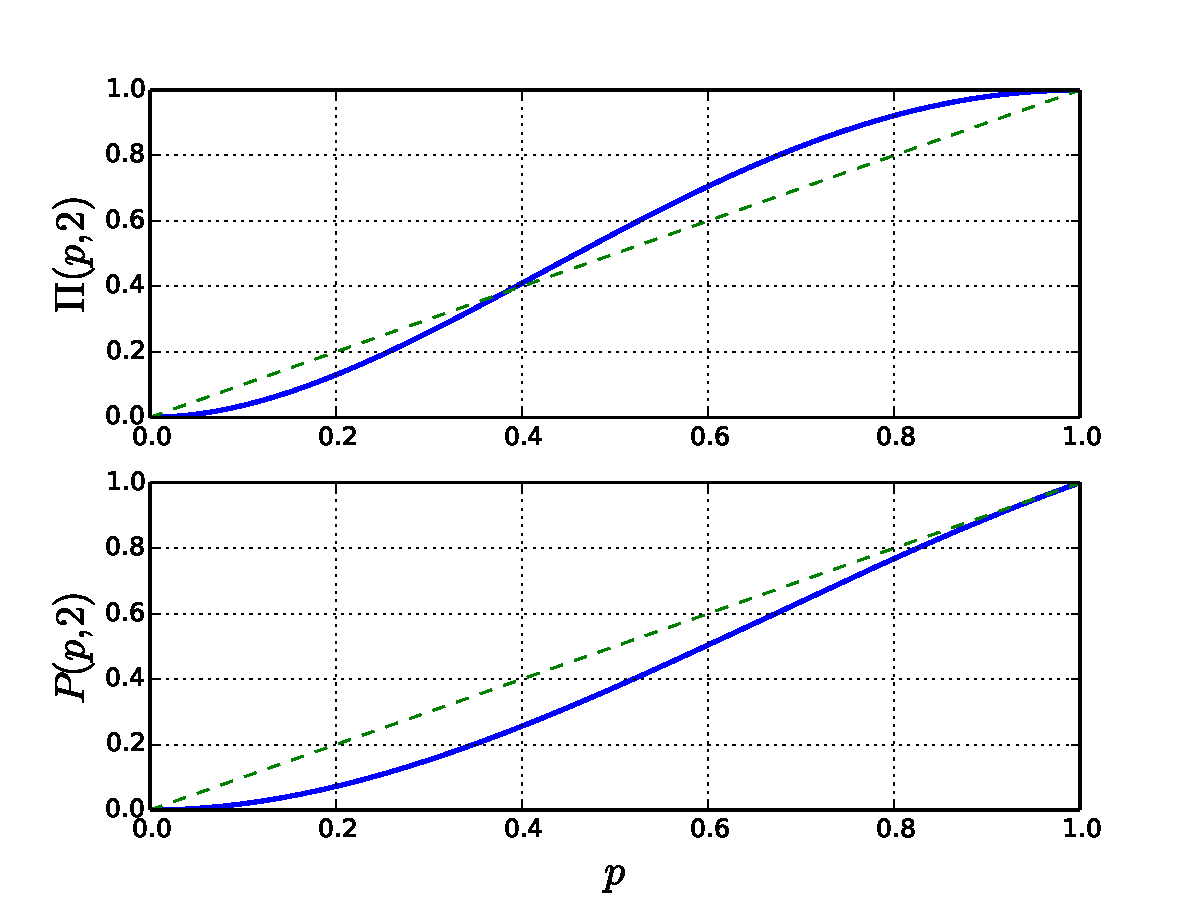
\includegraphics[width=\textwidth]{11.pdf}
\end{figure}

\newpage
We note some things about the curves: Both curves start at $0$ for $p=0$ and go to $1$ as $p\to 1$, this is very intuitive. They are also completely smooth. Note that the spanning cluster density is always below $p$, this makes perfect sense. The spanning cluster density is the probability of a random site to be a part of the spanning cluster. Now, the random site doesn't \emph{have} to be occupied, so the highest-estimate for $P$ should always be $p$---and occupied sites don't have to be part of a spanning cluster. In this case, if there \emph{is} a spanning cluster, all occupied sites automatically belong to it, so it is not surprising that the the difference from $p$ dies out as $\Pi\to 1$. For larger clusters however, it is very possible to have both a spanning cluster, and non-spanning cluster in the same experiment.

We are more interested in $P(p, \infty)$ than $P(p, 2)$ but having the probabilities on closed form for small $L$ let's us verify our solvers in a clean manner.

\subsection*{Measuring $\Pi(p,L)$ and $P(p, L)$ numerically}

For larger lattices, listing all the possible configurations becomes impossible due to the sheer number of them. Instead we do monte carlo simulations. By generating $N$ matrices of size $L$ and checking them against the probability $p$, we can look at the number of them that are percolating, the ratio of percolating systems to the total number of systems simulated gives an estimate for $\Pi(p,L)$ that improves as $N$ improves.

If we simulate $N$ systems, and find that $n$ of them are percolating, and they have total mass of $M$ we can estimate 
$$\Pi(p,L) = \frac{n}{N}, \qquad P(p,L) = \frac{\sum_i M_i}{NL^2}.$$

\clearpage

%%%%%%%%%%%%%%%%%%%%
%%%  QUESTION 12 %%%
%%%%%%%%%%%%%%%%%%%%

\section{ Cluster number density in 1-d percolation}
\begin{itemize}
	\item Define the cluster number density for 1-d percolation
	\item Show how it can be measured.
	\item Discuss the behavior when $p \to p_c$. How does it relate to your simulations in two-dimensional systems?
\end{itemize}

\subsubsection*{Definition of number cluster density}

In a random system, there can be many different clusters, of varying sizes. For a large system, when $p > p_c$ there will usually be one or more spanning cluster, but also many non-spanning clusters. When $p < p_c$ there will usually just be many non-spanning clusters. We might ask the question how the sizes of the clusters are distributed, and how that distribution changes as $p \to p_c$. The cluster number density is part of this distribution, the probabilty of a random site to belong to a cluster of size $s$ will be given by
$$p(s) = sn(s,p),$$
here $n(s,p)$ is the cluster number density. It is the probability of a random siste in the matrix to be a specific in a cluster of size $s$. The normalization requirement on the number cluster density is
$$P(p) + \sum_s s n(s,p) = p,$$
Where $P$ is the spanning cluster density. We can understand the normalization requirement, as any random site is only occupied with probability $p$ and will then either be part 
of the finite cluster of size $s$ or part of the infinite spanning cluster. Note that this implies that we \emph{do not} count the spanning cluster for the cluster number density (even for finite spanning clusters).

\subsubsection*{The spanning cluster density in 1D}
In 1D we can easily find the spanning cluster density on closed form, it will be
$$n(s,p) = p^s (1-p)^2.$$
This is because $s$ sites must be occupied, and the left neighbor and right neighbor must be unoccupied.

\subsubsection*{Measuring cluster number density}

We can estimate the cluster number density through simulation, by generating a percolating system, and counting the number of clusters of size $s$, we can then estimate the cluster number density from
$$\overline{n(s,p)} = \frac{N_s}{L^d}.$$
A better estimate is of course found by repeating the experiment many times
$$\overline{n(s,p)} = \frac{N_s(M)}{ML^d}.$$
For a large system, $s$ can have very many different values, so we need to bin the results into a histogram. However, it turns out that the cluster number density is a distribution with fat tails, to then meaningfully capturing large clusters, and not having many empty bins, we should implement logarithmic binning, meaning the bins increase in size exponentially as $s$ growns---it is then \emph{vital} to divide by the correct bin width!

\subsubsection*{Behaviour as $p \to p_c$}

To study the behaviour when $p\to p_c$, we rewrite the cluster number density. First we consider $p$ to be constant, and only look at the $s$-dependance of $n$.
$$n(s,p) = (1-p)^2 G(s), \qquad G(s) = p^s = e^{s \ln p} = e^{-s / s_\xi}, \qquad s_\xi = -\frac{1}{\ln p}.$$
Here $s_\xi$ is the characteristic cluster size. We see that
$$G(s) = \begin{cases}
	1 & \mbox{for } s \ll s_\xi, \\
	0 & \mbox{for } s \gg s_\xi, \\
\end{cases}.$$
So it is likely that our system has clusters smaller than the characteristic cluster size, but not many clusters larger than it. 

Now, the only $p$-dependance in $G(s)$ is through $s_\xi$, and we find that $s_\xi$ diverges as $p\to 1$, this is because $p_c = 1$ in 1D. As $p \to 1$ we can rewrite 
$$s_\xi \simeq \frac{1}{1-p},$$
And so we see that $s_\xi$ diverges as a power law when $p \to p_c$, this will be the case in any dimensionality
$$s_\xi = |p-p_c|^{-1/\sigma}.$$
This divergence obviously only occurs in infinite systems. It is easily understood, as we approach $p_c$, the system is getting close to percolating, and so we are getting larger and larger clusters, when the system becomes percolating, the spanning cluster stars eating away the big clusters, and so the characteristic cluster size falls down again.

We can measure $\sigma$ by finding $s_\xi$ for different $p$ as $p \to p_c$. Hopefully $s_\xi$ follows a power law. There is a challenge here involved with our system being finite. We could also use data collapse, if we plot the different $n(s,p)$ curves as functions of $s/s_\xi$, we could try different $\sigma$ values untill all the curves collapse to a universal curve, this is the correct $\sigma$ value.

In two-dimensional systems, $s_\xi$ also diverges. But here we start to distingiush between the mass of a cluster, and its extent. So we distinguish between $s_\xi$ and $\xi$. Both diverge, but $s_\xi$ scales faster
$$s_\xi \propto \xi^{D}, \qquad D < d.$$ 

\clearpage

%%%%%%%%%%%%%%%%%%%%
%%%  QUESTION 13 %%%
%%%%%%%%%%%%%%%%%%%%

\section{Correlation length in 1-d percolation}
\begin{itemize}
	\item Define the correlation length $\xi$ for 1-d percolation.
	\item Discuss its behavior when $p \to p_c$. 
	\item How is it related to cluster geometry and your results for twodimensional percolation?	
\end{itemize}

\subsubsection*{Correlation length $\xi$}

We start of by definint the correlation function $g(r)$, which is the probability of two occupied sites a distance $r$ apart of being connected---the $r$ coordinate is an integer argument denoting the number of sites inbetween. In 1D, this is quite simple to compute, it is simply
$$g(r) = p^r = e^{r \ln p} = e^{-r/\xi}, \qquad \xi = -\frac{1}{\ln p},$$
where $\xi$ is the correlation length. We see the correlation length is a cut-off for the correlation function, in the sense that
$$g(r) = \begin{cases}
	1 & \mbox{for } r \ll \xi, \\
	0 & \mbox{for } r \gg \xi.
\end{cases}$$
So it is reasonable to find clusters of extent $\xi$ and smaller in a given system, but not much larger than $\xi$.

\subsubsection*{Divergence of $\xi$}
To study the $p\to p_c$ we realize that in 1D, $p_c = 1$ and rewrite
$$\xi = -\frac{1}{\ln p} = \frac{1}{p-1} = (p-p_c)^{-\nu}.$$
So we see that $\xi$ diverges towards infinity when $p \to p_c$, this is true for any dimension, but the exponent changes. This behaviour makes a lot of sense. As $p \to p_c$ the system is getting close to percolating, and so there will be very large (but still finite) clusters, untill we hit $p=p_c$ where the spanning cluster forms, which is infinite in extent.

\subsubsection*{Cluster geometry}

In 1D, the correlation length $\xi$ is exactly the same as the characteristic cluter size $s_\xi$. This is because extent/length is the same as mass in 1D. In 2D however, we have to clarify what we are talking about, because a cluster of mass $s$ can have very many different shapes. In 2D, we must carefully distingiush between the correlation length $\xi$ and the characteristic cluster size $s_\xi$, as they will be different. The correlation length tells us the extent of the system, and is therefore important for the finite scaling theory, as it is the ratio $\xi/L$ that tells us wether the finite size of our system affects our results.

We know that
$$s_\xi \propto \xi^D, \qquad \mbox{where } D \mbox{ is a fractal dimensionality constant } D < d.$$

Another property we use to quantify the geometry of a cluster is the radius of gyration, it is the variance of the clusters sites to it's centre of mass
$$R_i^2 = \frac{1}{s_i}\sum_{n=1}^{s_i} (\vec{r}_i - \vec{R}_i)^2.$$
Where $R_i$ is the radius of gyration for a given cluster $i$, $s_i$ is the cluster size, $n$ is a site label, $\vec{r}$ is the site location and $\vec{R}_i$ is the clusters centre of mass.

For two clusters of equal mass, the radius of gyration will be smaller for the denser cluster, and larger for the sparser cluster. We know that 
$$s \propto R_s^D.$$

\begin{align*}
s_\xi &\propto |p-p_c|^{-1/\sigma}, \\
s_\xi &\propto \xi^D = |p-p_c|^{-D\nu}, \\
D\nu\sigma &= 1.
\end{align*}

\begin{center}
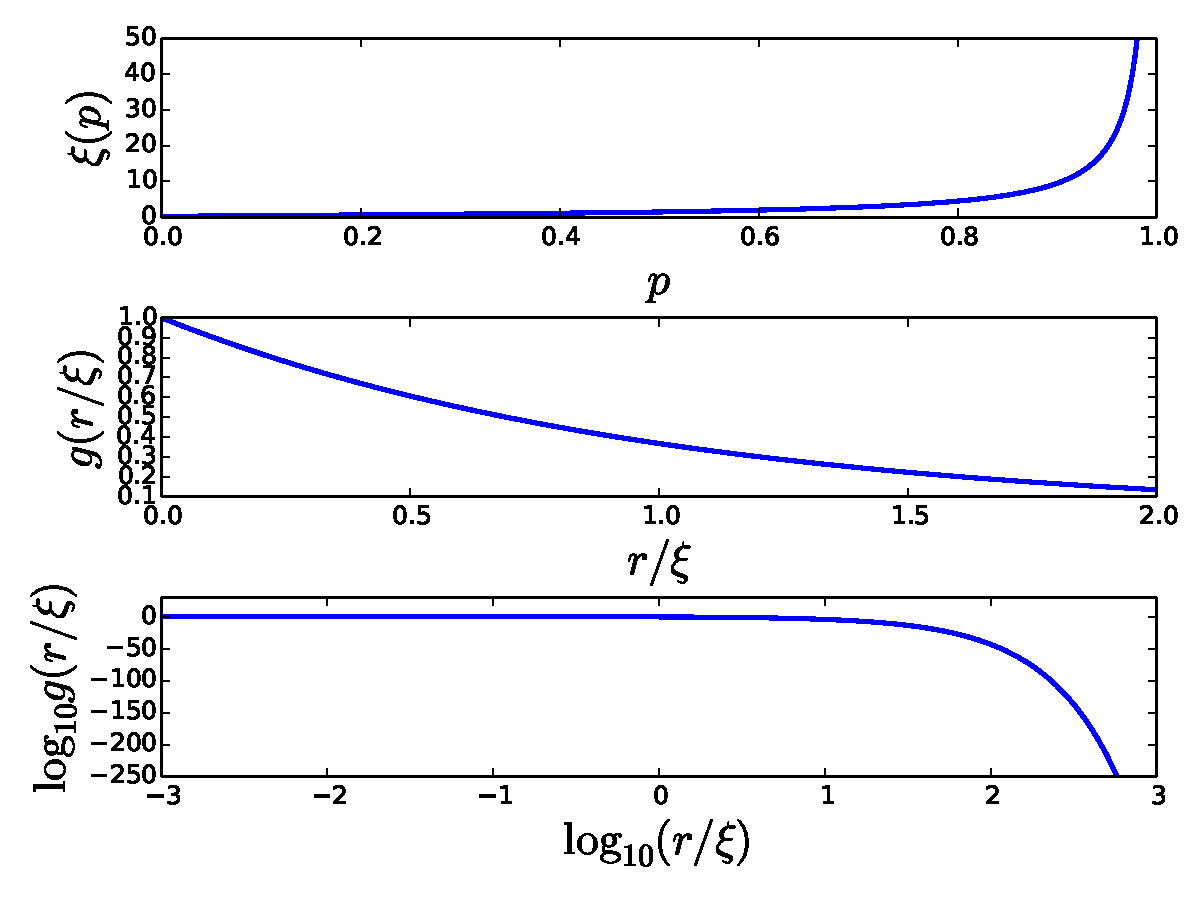
\includegraphics[width=0.8\textwidth]{13.pdf}
\end{center}


\clearpage

%%%%%%%%%%%%%%%%%%%%
%%%  QUESTION 14 %%%
%%%%%%%%%%%%%%%%%%%%

\section{Cluster size in 1-d percolation}
\begin{itemize}
	\item Introduce the characteristic cluster size for the 1-d percolation problem.
	\item Discuss their behavior when $p \to p_c$.
	\item Relate to your simuluations on 2-d percolation.
\end{itemize}


A random system will have clusters of varying shapes and sizes. In 1D percolation, all clusters of the same size look the same. The cluster number density is the probability for a given site to be a specific site of a cluster of size $s$, so the probability density of cluster sizes is given by
$$sn(s,p).$$
If we focus only on the cluster number density, in 1D it becomes
$$n(s,p) = (1-p)^2 p^s.$$
Now, the $(1-p)^2$ is constant for a constant $p$, so it isn't that important, but we have
$$p^s = e^{s \ln p} = e^{-s/s_\xi}, \qquad s_\xi = -1/\ln p,$$
and this is the characteristic cluster size $s_\xi$. Not that $n(s,p)$ is pretty constant when $s < s_\xi$ but that it quickly dies out when $s > s_\xi$. It doesn't matter that the probability of a given site to be occupied is multiplied by $s$, as $n(s,p)$ dies out exponentially when $s > s_\xi$, and $s$ only grows linearily.

So the characteristic cluster size is the biggest cluster size it is reasonable to find in our random system.

\subsubsection*{When $p \to p_c$}
Now, let's study the definition of $s_\xi$
$$s_\xi = -\frac{1}{\ln p}, \qquad p\in [0,1] \To s_\xi \in [0, \infty].$$
So the characteristic cluster sizes diverges when $p \to 1$. The reason for this is that $p_c=1$ for the 1D system. So that as $p\to 1$ we are expecting bigger and bigger clusters to form, but as long as $p = 1-\eps$ for a finite  $\eps$, the infinite 1D cluster hasn't started percolating.

\subsubsection*{Comparison with 2D}

In 2D, the characteristic cluster size talks about the total \emph{mass} of clusters, that means, the total number of sites in the cluster. It does not take into account the shape or geometry of the cluster. In 1D we found that the characteristic cluster size diverges as a power law as $p\to p_c$, this same behaviour is observed in 2D, but with a different power constant
$$s_\xi = |p-p_c|^{-1/\sigma}.$$
(Note that $\sigma < 1$, so the characteristic cluster size diverges \emph{faster} in 2D). The reason for divergence is exactly the same in 2D. As long as $p < p_c$, there is no spanning cluster, but as $p$ is getting very close, we are getting very large, but still \emph{finite}, clusters. As $p=p_c$, the system starts percolating and forms a spanning cluster, meaning $s_\xi$ `reached' infity. As $p > p_c$ we see an exact reversed trend, where $s_\xi$ goes back down, this is because the characteristic cluster size is connected to the cluster number density and is only used to describe the fintie (non-spanning) clusters, so as $p > p_c$ and $p$ increases, the added probability causes the spanning cluster to grow in size, and it `swallows' other finite clusters. The bigger a finite cluster is, the bigger the probability of it being swallowed by the spanning cluster, so it makes sense that $s_\xi$ decreasing as a power law. As $p \to 1$, we should obviously have $s_\xi \to 0$ as the probability of any finite clusters is 0. So we see that the power law doesn't hold, but this isn't surprising as the power law is only valid when $|p-p_c|$ is small, we used a Taylor expansion to first order.

\subsubsection*{Geometry}

In 2D, there clusters will also have different geometries, so in addition to the characteristic cluster size, we might look at the \emph{extent} of a closter, we then define the correlation length $g(r)$, which will have a cut-off at the correlation length $\xi$. So in 1D we have $s_\xi = \xi$, but in 2D
$$s_\xi \propto \xi^{D}, \qquad D < d.$$
We can also look at the radius of Gyration, which is defined as
$$R_i^2 = \frac{1}{s_i}\sum_{n=1}^{s_i} (\vec{r}_i - \vec{R}_i)^2.$$
So it can be interpreted as the variation in the distance to the centre of mass of the cluster. One can also show that
$$R_s^2 \propto s_\xi^D.$$

\subsubsection*{In our simulation}

In our simulations, we found the cluster number density $n(s,p)$ by logarithmic binning of all the cluster sizes in the system.


\clearpage

%%%%%%%%%%%%%%%%%%%%
%%%  QUESTION 15 %%%
%%%%%%%%%%%%%%%%%%%%


\section{Measurement and behavior of $P(p, L)$ and $\Pi(p, L)$}
\begin{itemize}
\item Discuss the behavior of $P(p, L)$ and $\Pi(p, L)$ in a system with a finite system
size $L$.
\item How do you measure these quantities?
\end{itemize}

\subsubsection*{Definition}

The percolation probability $\Pi(p, L)$ is the probability of a random system of size $L$ to have at least 1 spanning cluster, when every site is inhibited with probability $p$. The spanning cluster density $P(p,L)$ is the probability a given site has of being a part of the spanning cluster, it is called the spanning cluster density, because it is equal to the average spanning cluster mass divied by the number of sites in the system. A system of `size' $L$ is different in 1D and 2D.

\subsubsection*{The behaviour of $P(p, L)$ and $\Pi(p, L)$}

Let us start at $L=\infty$. When the system is infite in size, there is a given value $p_c$ where the system will always start to percolate. In 1D it is obvious that $p_c = 1$, since a single unihabited site will prevent a spanning cluster from forming. In 2D it is $p_c = 0.59275$. The percolation probablity $\Pi(p,L)$ is then simply a step function at $p=p_c$.  For the other extreme, $L=1$, the 1D and 2D cases are the same, and we get the linear curve $\Pi(p, 1) = p$ in both cases. 
\begin{center}
	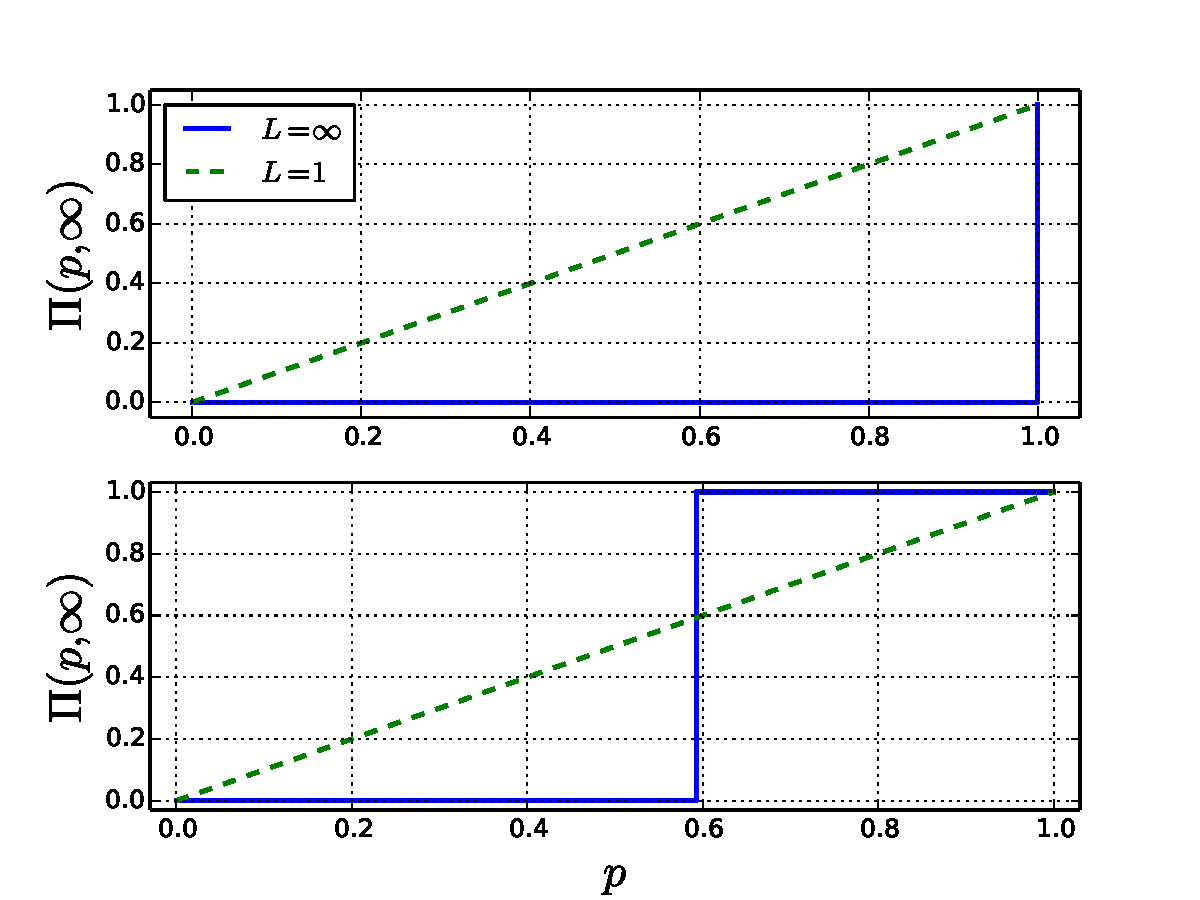
\includegraphics[width=0.7\textwidth]{15.pdf}
\end{center}

Now, let us look at small, but finite $L$. In 1D, the probability is easy to find
$$\Pi(p,L) = p^L,$$
And we see that as $L$ grows, it quickly dies out for small $L$. When $p \to 1$ the probability goes to 1, the bigger the system, the steeper this slope is. So the probability is a monotonely decreasing function as $L$ grows. This is very intuitive: for the system to be percolating, we have to `get lucky' and get every site occupied. For a small $L$ this is very doable, but as $L$ grows, it becomes impossible. You can throw a 5-dice yahtzee, but you can't throw a million-dice yahtzee.

\begin{center}
	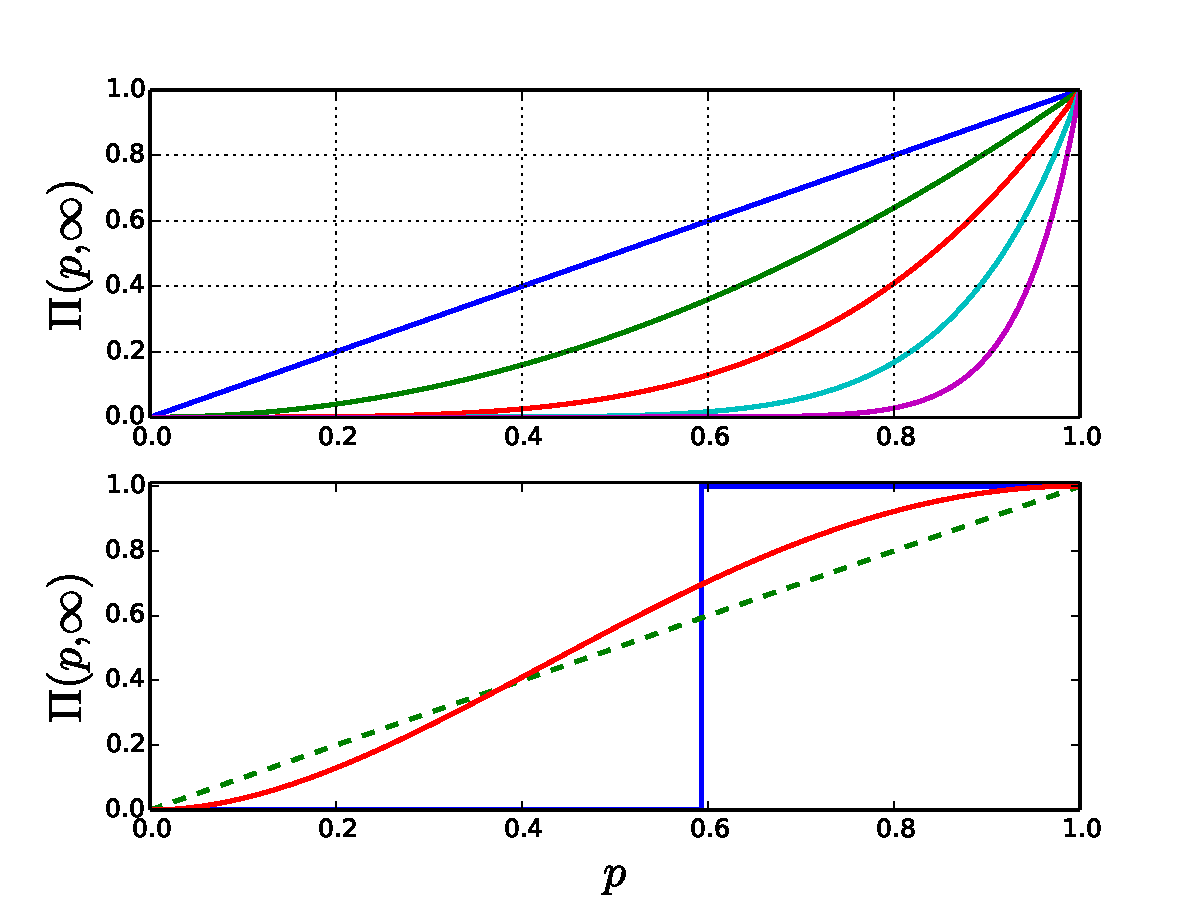
\includegraphics[width=0.7\textwidth]{15b.pdf}
\end{center}

For 2D, there is no easy expression for the percolation probability as function of $L$, but for the smallest $L$ we can tabulate all possible configurations, weight them according to their probabilities, and then find the expection value for the percolation probability by summing over them (and their weights). The number of configurations grows as $2^{L\times L}$, so it grows exponentially with the system size. Let us quickly show $L=2$ as an example, there are 16 configurations, of these, 9 are percolating

\begin{center}
$4\times$
\begin{tabular}{|c|c|}
  \hline
  \ \ \cellcolor{black}&  \ \ \  \\ \hline
  \ \ \cellcolor{black} & \qquad \\
  \hline
\end{tabular} \qquad
\qquad $4\times$
\begin{tabular}{|c|c|}
  \hline
  \  \cellcolor{black} & \cellcolor{black} \ \ \  \\ \hline
  \ \  \cellcolor{black} & \qquad \\
  \hline
\end{tabular} \qquad 
\qquad $1\times$
\begin{tabular}{|c|c|}
  \hline
  \ \ \cellcolor{black} & \cellcolor{black} \ \ \  \\ \hline
  \cellcolor{black} & \cellcolor{black} \qquad \\
  \hline
\end{tabular}	
\end{center}
So from this we get
$$\Pi(p, 2) = 4p^2(1-p)^2 + 4p^3(1-p) + p^4, \\$$

We see that close to $p=0$ and $p=1$, the function is starting to `glue' to the correct $P=0$. As we increase $L$, we see this trend continues, giving a sharper and sharper slope. We can interpret this phenomena much like that for 1D. In the infinite lattice, we need $p=p_c$ to percolate, and we will always percolate above $p_c$. In a finite lattice however, we can get `lucky', and just happen to get a percolation cluster at $p \leq p_c$, just like for 1D, in 2D however, we can also be `unlucky', in that we might not have a spanning cluster even for $p > p_c$. As $L$ grows, the chance of being `lucky' and `unlucky' both become smaller and smaller, and in the $L\to \infty$ limit, we cannot be either lucky or unlucky anymore, we have the step function.


\subsubsection*{Measurement}

The idea to find $\Pi(p, L)$ for small $L$ was to list all configurations and then find the expected value by taking the sum of configurations weighted by their probabilities. For big $L$, this isn't possible, since there are two many possible configurations. However, if we create a random matrix, this is the same as sampling configuration space, drawing out a configuration at random. If we draw out $N$ samples, and $N_p$ of them are percolating, we can then estimate the percolation probability from
$$\Pi(p, L) \simeq \frac{N_p}{N}.$$

To create a random matrix, we draw a $L\times L$ matrix of random numbers uniformly distributed in $[0,1]$. Then we check every site against the preset $p$, any site with value less than $p$ is inhabited, every site with value more than $p$ is not inhabited.
 

\clearpage

%%%%%%%%%%%%%%%%%%%%
%%%  QUESTION 16 %%%
%%%%%%%%%%%%%%%%%%%%

\section{The cluster number density}
Introduce the cluster number density and its applications: Definition, Measurement, Scaling, Data-collapse.

\subsubsection*{Definition}

Let us consider a $L\times L$ system. Every site is occupied with probability $p$, for a big cluster this means that $p$ is the porosity. A system will contain many clusters of varying sizes, and perheps one or more spanning clusters. The cluster number density gives the probability distribution of the finite clusters, we have the normalization 
$$\sum_s sn(s,p) + P(p) = p,$$
Here, $P(p)$ is the spanning cluster density, and $sn(s,p)$ is the probability of a random site to belong to a cluster of size $s$. Note that the probability is given as $s n(s,p)$ so $n(s,p)$, which is the cluster number density can be defined as the probability of a random site in system to be a specific site in a cluster of size $s$.

\subsubsection*{Measurement}

We generate a $L\times L$ percolation system. We label all clusters and find their masses. Once we have all clusters and their masses (we do \emph{not} include the spanning cluster), we can estimate the cluster number density from
$$\overline{n(s,p)} = \frac{N_S}{L^{d}},$$
where $N_S$ is the number of clusters of site $S$. Usually we want to do this many times, to get better data, so we generate $M$ such systems, and keep track of the running total of clusters of size $s$.
$$\overline{n(s,p)} = \frac{N_S(M)}{ML^{d}}.$$
Note that we only count the number of clusters of size $s$, we do not count their masses, this is beacuse we are looking for $n(s,p)$ alone, \emph{not} $sn(s,p)$. Now, there are very many different possible values of $s$, so we want to use binning, Meaning we combine results for close-lying $s$-values. This gives us a histogram that estimates the probability density $n(s,p)$. However, it turns out $n(s,p)$ is a probability density with a fat tail, meaning large $s$-values are not very likely, but more likely than in a expoential distribution (so called Black Swan behaviour of power laws). If we use uniform bin sizes, this means we will have very many bins without any hits in them! To solve this problem, we use logarithmic binning, meaning we let the bins grow in size as we get larger and larger $s$-values, in an exponential fashion. When using non-uniform bin sizes, we must remember to divide by the correct bin size to get the right probability density in the end, or the tail ends of the probability density would become exponentially overexposed.

\subsubsection*{Scaling}
To describe the scaling of the cluster number density, let us consider the 1D case, where the CND is known on closed-form
$$n(s,p) = (1-p)^2 p^s = (1-p)^2 e^{s \ln p} = (1-p^2) e^{-s/s_\xi}.$$
Now, for a constant $p$, the first term is just a normalization, so the exponential term describes the scaling. We see that it is relatively flat as long as $s \ll s_\xi$, but drops of exponentially as $s > s_\xi$. Here $s_\xi$ is called the characteristic cluster size, it can be rewritten to
$$s_\xi = -\frac{1}{\ln p} = \frac{1}{1-p} = |p-p_c|^{1/\sigma}.$$
This result is true in all dimensions, so the characteristic cluster size diverges as $p\to p_c$ as a power law. This means the behaviour of $n(s,p)$ where $p \neq p_c$ is only similar to that when $p=p_c$ when $s \ll s_\xi$. We can describe this by introducing a cut-off function
$$n(s,p) = s^{-2} \bigg(\frac{s^2}{s_\xi^2} e^{-s/s_\xi} \bigg) = s^{-2} F\bigg(\frac{s}{s_\xi}\bigg).$$
So we have baked the $s_\xi$ dependence into the cut-off function, so we have
$$n(s,p) = n(s,p_c) F\bigg(\frac{s}{s_\xi}\bigg).$$
This is true in general. Where
$$n(s,p_c) = Cs^{-\tau}, \qquad s_\xi = s_0|p-p_c|^{-1/\sigma}, \qquad F\bigg(\frac{s}{s_\xi}\bigg)\to 0 \mbox{ for } s\gg s_\xi.$$

\subsubsection*{Data collapse}
As we all $p$-dependence has been put into $F(s/s_\xi)$ through the characteristic cluster size $s_\xi$, the cut-off function should be universal for all $p$ if we plot it as a function of $s/s_\xi$. This is what is known as a data collapse. As we can gather data from simulations for a lot of different $p$, which will give curves that are different, but if we plot it in a manner that takes into account the $p$-dependence, all our data should `collapse' into a universal curve. Now, there will some small deviations due to noise, but the curves should be very similar. If there are systematic deviations, we know there is some systematic error in our program.


\clearpage

%%%%%%%%%%%%%%%%%%%%
%%%  QUESTION 17 %%%
%%%%%%%%%%%%%%%%%%%%

\section{Finite size scaling of $\Pi(p, L)$}
\begin{itemize}
	\item Discuss the behavior of $\Pi(p, L)$ in a system with a finite system size $L$.
	\item How can we use this to find the scaling exponent $\nu$
	\item And the percolation threshold, $p_c$?
\end{itemize}

In a numerical simulation, we are forced to work with a finite system size $L$, but we are usually looking for results in the thermodynamic limit, i.e., the infite lattice. Thus, we need some theory to extrapolate infinite-size predictions from our finite size results. One such theory is finite size scaling, where we look at how our results scale with the system size, and use that as a predictor.

One of the fundamental properties when looking at size scaling is the correlation length, $\xi$, it can be interpreted as a cut-off value for the distribution in the extent of clusters. So in a system with correlation length $\xi$, we expect to find clusters of size (measured in extent, not mass) all the way up to roughly $\xi$, but not many clusters larger than this. When $p$ is close to $p_c$, we know that the correlation length diverges as a power law
$$\xi \propto |p-p_c|^{-\nu}.$$

Now, for any system where $\xi \ll L$, our system does not really notice the finite size, as there are no clusters larger than the system size, it isn't really `truncated'. So if we see our system as a cut-out of an infinite lattice, we haven't sliced any large clusters to get our subsystem. When $\xi \gg L$ however, the clusters in our systems are supposed to be much larger, and so our results will look very different. 

\subsubsection*{The percolation probability}
In the thermodynamic limit, we know the percolation probability is a step-function at $p=p_c$. For lower $L$, it will be `smeared' out. If we consider how it is affected by the finite size of our lattice, it makes sense that
$$\Pi(p, L) = \begin{cases}
	1 & \mbox{for } \xi \gg L \\
	0 & \mbox{for } \xi \ll L.
\end{cases}.$$
In any case, it is obvious that it should scale as a function of $L/\eps$, in 1D we can find this function analytically, and it is simply
$$\Pi(p, L) = f\bigg(\frac{L}{\xi}\bigg) = e^{-L/\xi}.$$
In 2D we can't find it analytically, but we don't need the exact form, we just need to know that it is some scaling relation of the $L/\xi$ ratio is enough. We write
$$\Pi(p, L) = f\bigg(\frac{L}{(p-p_c)^{-\nu}}\bigg) = \Phi\big((p-p_c)L^{1/\nu}\big).$$
What we have found here, is a relation of how the percolation probability should scale with $p$ and $L$. To use this relation for something useful, we flip the question slightly and say: If we want a specific value for the percolation probability, let's say 60 \%, what does $p$ need to be? This answer of course depends on $L$
$$\Pi(p_{\pi=x}(L), L) = x.$$ 

We can then find
$$(p_{\pi=x} - p_c)L^{1/\nu} = \Phi^{-1}(x).$$
Now, we don't know the exact form of $\Phi$, but we know it is a smooth function that goes from 1 to 0, so an inverse should exist, and so we just dub it some constant
$$p_{\pi=x}(L) = p_c + C_x L^{-1/\nu}.$$
There are three unknowns here, but we can still predict both $p_c$ and $\nu$, but how? First we look at the difference in two $x$ values. Taking the logarithm gives
$$\log \Delta p(L) = \log (C_{x_2} - C_{x_1}) - \frac{1}{\nu} \log L.$$
And so if we measure $\Delta p(L)$ numerically for various $L$, and plot it in a log-log plot, we should get a straight line with slope $-1/\nu$. And now we can plot $p_{\Pi=x}$ as a function of $L^{-1/\nu}$. which gives a straight line
$$p_{\Pi = x}(L^{-1/\nu}) = p_c + C_x L ^{-1/\nu},$$
So the slope depends on the unknown $C_x$, but it is the intersect with the $y$-axis that gives $p_c$. Linear regression thus gives $p_c$.

\subsubsection*{Summary}

It is almost trivial to find $\Pi(p, L)$ for finite $L$ numerically, we can just generate many systems, and count the number that are spanning. However, we are really interested in the thermodynamic limit $L\to \infty$, and it is not immedietly apparent how we go from finite $L$ to infinite $L$. By looking at how $\Pi$ should scale as a function of $\xi/L$, we found a finite size scaling relation, that let us predict the percolation probablity $p_c$ and the scaling parameter $\nu$, which both are values from the thermodynamic limit.


\clearpage

%%%%%%%%%%%%%%%%%%%%
%%%  QUESTION 18 %%%
%%%%%%%%%%%%%%%%%%%%

\section{ Subsets of the spanning cluster}
\begin{itemize}
	\item Introduce and discuss the scaling of subsets of the spanning cluster.
	\item How can we measure the singly-connected bonds, and how does it scale?
\end{itemize}

\subsubsection*{Subsets of the spanning cluster}

If we have a percolating system, there is a spanning cluster---if we want to analyze the spanning cluster closer, we divide it into subsets, these are
\begin{itemize}
	\item The single connected bonds
	\item The backbone
	\item The dangling ends
\end{itemize}

It is easiest to understand these subsets by envisioning flow through the spanning cluster. 

The singly connected bonds are the bottlenecks in the system, they are the sites that would make the cluster non-spanning if they were removed. Any flow through the spanning cluster \emph{must} go through the singly-connected bonds.

The backbone are any sites that the flow can use to move from one side to the other through the spanning cluster. It is the same as the transport-available porosity in nano-porous materials. Note that the definition of the backbone includes the singly connected bonds.

Lastly, the dangling ends are the `dead ends', they are parts of the spanning cluster with only one site leading into them, if that site is removed, the dangling end is cut off. This means the dangling end won't contribute to any flow through the system, as in a stationary flow scenario, there can be now flow into or out of a dangling end.

\subsubsection*{Scaling of the subsets}

Let us look at how these subsets scale for an increasing system size. We know that the mass of the spanning cluster itself follows a power law
$$M \propto L^D, \qquad D \leq d.$$
Where $D$ is the fractal dimension of the spanning cluster, which should be a power of $p$. In the limit $p\to 1$, we expect $D \to d$ as the spanning cluster would grow as quickly as the system itself. And if $p$ is smaller, we expect $D < d$ as a fraction of all the sites added when increasing the system size will go to unoccupied sites, or non-spanning clusters.

It turns out that the mass of the subsets of the spanning cluster all individually follow similar power laws, but with different critical exponent
$$M_i \propto L^{D_i}, \qquad i \in \{\mbox{SCD}, \mbox{BB}, \mbox{DE}\}.$$
The question is what the fractal dimensionalities are. We can quickly find some restrictions
$$M_i \leq M \quad \To \quad D_i \leq D.$$

If we let SAWs walk from on end of the spanning cluster to the other, they can follow many different paths. Any SAW that enters a dangling end gets stuck. The SCBs can be given as the intersect of all SAW paths that make it through, while the backbone is the union of all SAW paths that make it through. If we then consider the scaling of the minimal and maximal SAW paths we find
$$D_{SC} \leq D_{\rm min} \leq D_{\rm max} \leq D_{BB} \leq D \leq d.$$

For $p=p_c$ in 2D, we find

\begin{center}
\begin{tabular}{c c c c c}
$D_{SC}$ & $D_{\rm min}$ & $D_{\rm max}$ & $D_{BB}$ & $D$ \\ \hline
3/4	& 1.1 & 1.5 & 1.6 & 1.89
\end{tabular}
\end{center}

Finally there are the dangling ends, we know that $D_{DE} \leq D$ and $D_{BB} \leq D$, but interestingly enough, both can't be less than $D$ at the same time, because this would cause to little growth of the spanning cluster as $L \to \infty$. So we see that the dangling ends grows quicker than the backbone as we approach the thermodynamic limit.

\subsubsection*{Measurement}

We could of course estimate the scaling of the subsets of percolating cluster by generating systems for various $L$ and simply looking at the masses of the subsets. We then need to have smart way to find these subsets. Let us look at the singly-connected bonds as an example. If we let a Left-walker and a Right-walker start at the same end of the cluster, they will both make it through. Taking the intersect of their paths will give us all the singly-connected bonds, as these are sites they both passed through, it is basicly the sandwich theorem. When doing this, one finds the scaling of the SCBs to be $1/\nu = 3/4$ in 2D. In our project 3, we did this with surprisingly good results.

One could also use renormalization theory to make theoretical arguments about the critical exponents and thus the scaling of the subsets. This is because the spanning cluster is a self-fractal. However, we didn't really go into detail on this, so I won't talk much about it.


\clearpage

%%%%%%%%%%%%%%%%%%%%
%%%  QUESTION 19 %%%
%%%%%%%%%%%%%%%%%%%%

\section{ Random walks / Flow in a disordered system}
\begin{itemize}
\item[Either:] Discuss the scaling theory for the distance $r^2(t)$ of a random walker
dropped at a random occopied site on either (1) the percolation system or (2)
the spanning cluster. (You can choose which case to discuss). Relate the results
to diffusion in a bulk fluid and in a nanoporous system.
\item[Or: ] How do you measure the conductivity of the spanning cluster? Discuss the
scaling theory for the conductivity $\sigma(p, L)$
\end{itemize}


\subsubsection*{Conductivity of the spanning cluster}

Conductance is the inverse of resistance. An electrical component will have a given conductance, which is a quantifier of how willing the component is at letting flow pass through it, this is described by Ohm's law
$$I = \frac{V}{R} = GV,$$
The current through the component is proportional to it's conductance $G$.

Conductivity is similar to conductance, but it is a material property, while conductance is a component property. So copper has a conductivity, but a given piece of copper wire has a conductance. For a 2D quadratic system, these are actually equal.
$$G = \sigma\frac{A}{L} = \sigma\frac{L^{d-1}}{L} = \sigma.$$

Instead of electric current, we use flow, which is described by Darcy's law
$$\Phi = \frac{k A}{\mu L} \Delta P.$$
Here $\sigma = k/\mu$ and $\Delta P$ is the pressure differential, which is similar to the voltage.

If we then apply a pressure differential to our system, and measure the flow through the entire system, we find the conductance. To find the flow through the entire system, we use Kirchoff's flow laws. The first flow law states that the total flow into and out of a site must equal zero, otherwise we would get a build-up of pressure in that site, which cannot be the case for stationary flow. So for any site $i$, we sum over the flow from the neighbors
$$\Phi_i = \sum_j g_{i,j} (p_j -p_i).$$
The flux $\Phi_i$ can only be non-zero at boundary sites, the conductance between neighbors is $\delta_{ij}$ so it is 1 for connected sites, and zero for others, and lastly the flow between sites is proportional to the pressure difference in them. Setting up this flow equation for all sites in our spanning cluster gives us a set of linear equations which we can write as the matrix-equation
$$Ap = c,$$
where $p$ is the pressure in all the sites, and $c$ is a vector describing the boundaries (the flow internally is zero, it is only non-zero on the boundaries). The matrix $A$ descrbies the cluster itself, it can be set up in a smart manner, making it sparse. We can solve the matrix equation to find $p$, giving us the pressure for all the sites in the cluster. The pressure tells us the flow between sites, and we can create a map of the flow through the system---this tells us if any given site is a dangling end, backbone or singly-connected bond. We can now find the conductance from
$$\sigma = \frac{\Phi}{\Delta P}.$$

\subsubsection*{Scaling theory of conductivity}

Let us look at the $p$-dependence first. It is obvious that the conductance should increase with $p$, as more and more volume becomes transport-available. One might assume that $\sigma$ should grow as $P$, it turns out however, that it grows faster! That might seem a bit strange, as the amount of transport-available porosity grows faster than the porosity itself, but this is only because there are many dangling ends when $p\simeq p_c$, and as $p$ grows, the dangling ends will become transport-available. We have
$$P \propto (p-p_c)^\beta, \quad \beta < 1, \qquad \sigma \propto (p-p_c)^\mu, \quad \mu > 1.$$

If we instead look at the system size dependence. Let us look at the conductance as a function of $\xi$ and $L$: $G(\xi, L)$. When $L \ll \xi$ the system will behave as it is close to $p = p_c$. When $L \gg \xi$ we can divide our system into subscells of size $\xi^d$ because it is self-similar (all subcells will look identical). Every subcell now appears to be close to $p = p_c$ and so every subcell will have conductivity $G(\xi, \xi)$. We then find the total conductance from
$$G(\xi, L) = \sigma \frac{A}{L} = G(\xi, \xi) \bigg(\frac{L}{\xi}\bigg)^{d-2}.$$
So in 2D, $G(\xi, L)$ remains constant as $L$ grows much larger than $\xi$, in 3D the conductance grows with growing $L$ indefinitely, as the area grows quadratically and the length of the sample only grows linearily. 


\end{document}



 
